\documentclass[aps,prd,reprint,preprintnumbers,showpacs,floatfix,nofootinbib,superscriptaddress]{revtex4-2}
\usepackage[utf8]{inputenc}
\usepackage{parskip}

\usepackage{amssymb}
\usepackage{amsmath}
\usepackage{mathtools}
\usepackage[dvipsnames]{xcolor}
\usepackage{xspace}
\usepackage{tabularx}
\usepackage{booktabs}
\usepackage{siunitx}
\usepackage{multirow}
\usepackage{subcaption}
\usepackage{graphicx}
\usepackage{xstring}
\usepackage{etoolbox}
\usepackage{notoccite}
\usepackage{natbib}
\usepackage{mathrsfs}
\usepackage{lineno}
\usepackage{tensor}
\usepackage{accents}
\usepackage{microtype}
\usepackage[justification=raggedright,singlelinecheck=false,format=plain]{caption}

\graphicspath{{figures/}}

\usepackage{tocbasic}
\setcounter{tocdepth}{1}
\DeclareTOCStyleEntry[numwidth=25pt,linefill=\bfseries\TOCLineLeaderFill]{tocline}{section}
\DeclareTOCStyleEntry[entryformat=\textit,numwidth=10pt,linefill=\TOCLineLeaderFill]{tocline}{subsection}
\DeclareTOCStyleEntry[entryformat=\textit,numwidth=10pt,linefill=\TOCLineLeaderFill]{tocline}{subsubsection}

\parindent 2mm

%MacrosJournalNames

% Journal names 
\def\aj{\rm{AJ}}
\def\actaa{\rm{Acta Astron.}}
\def\araa{\rm{ARA\&A}}
\def\apj{\rm{ApJ}}
\def\apjl{\rm{ApJ}}
\def\apjs{\rm{ApJS}}
\def\ao{\rm{Appl.~Opt.}}
\def\apss{\rm{Ap\&SS}}
\def\aap{\rm{A\&A}}
\def\aapr{\rm{A\&A~Rev.}}
\def\aaps{\rm{A\&AS}}
\def\azh{\rm{AZh}}
\def\baas{\rm{BAAS}}
\def\bac{\rm{Bull. astr. Inst. Czechosl.}}
\def\caa{\rm{Chinese Astron. Astrophys.}}
\def\cjaa{\rm{Chinese J. Astron. Astrophys.}}
\def\icarus{\rm{Icarus}}
\def\jcap{\rm{J. Cosmology Astropart. Phys.}}
\def\jrasc{\rm{JRASC}}
\def\memras{\rm{MmRAS}}
\def\mnras{\rm{MNRAS}}
\def\na{\rm{New A}}
\def\nar{\rm{New A Rev.}}
\def\pra{\rm{Phys.~Rev.~A}}
\def\prb{\rm{Phys.~Rev.~B}}
\def\prc{\rm{Phys.~Rev.~C}}
\def\prd{\rm{Phys.~Rev.~D}}
\def\pre{\rm{Phys.~Rev.~E}}
\def\prl{\rm{Phys.~Rev.~Lett.}}
\def\pasa{\rm{PASA}}
\def\pasp{\rm{PASP}}
\def\pasj{\rm{PASJ}}
\def\rmxaa{\rm{Rev. Mexicana Astron. Astrofis.}}
\def\qjras{\rm{QJRAS}}
\def\skytel{\rm{S\&T}}
\def\solphys{\rm{Sol.~Phys.}}
\def\sovast{\rm{Soviet~Ast.}}
\def\ssr{\rm{Space~Sci.~Rev.}}
\def\zap{\rm{ZAp}}
\def\nat{\rm{Nature}}
\def\iaucirc{\rm{IAU~Circ.}}
\def\aplett{\rm{Astrophys.~Lett.}}
\def\astropj{\rm{Astrophys.~J.}}
\def\apspr{\rm{Astrophys.~Space~Phys.~Res.}}
\def\bain{\rm{Bull.~Astron.~Inst.~Netherlands}}
\def\fcp{\rm{Fund.~Cosmic~Phys.}}
\def\gca{\rm{Geochim.~Cosmochim.~Acta}}
\def\grl{\rm{Geophys.~Res.~Lett.}}
\def\jcp{\rm{J.~Chem.~Phys.}}
\def\jgr{\rm{J.~Geophys.~Res.}}
\def\jqsrt{\rm{J.~Quant.~Spec.~Radiat.~Transf.}}
\def\memsai{\rm{Mem.~Soc.~Astron.~Italiana}}
\def\nphysa{\rm{Nucl.~Phys.~A}}
\def\nphys{\rm{Nucl.~Phys.}}
\def\physrep{\rm{Phys.~Rep.}}
\def\physscr{\rm{Phys.~Scr}}
\def\planss{\rm{Planet.~Space~Sci.}}
\def\procspie{\rm{Proc.~SPIE}}
\def\procrsa{\rm{Proc.~Math.~Phys.~Eng.~Sci.}}
\def\annmath{\rm{Ann.~Math.}}
\def\mathann{\rm{Math.~Ann.}}
\def\annphys{\rm{Ann.~Physics (N.~Y.)}}
\def\annderphys{\rm{Ann.~Phys.}}
\def\ptrsla{\rm{Philos.~Trans.~R.~Soc~A}}
\def\ptrslo{\rm{Philos.~Trans.~R.~Soc~I}}
\def\jmp{\rm{J.~Math.~Phys.}}
\def\cqg{\rm{Class.~Quantum~Gravity}}
\def\physrev{\rm{Phys.~Rev.}}
\def\foundphys{\rm{Found.~Phys.}}
\def\epjc{\rm{Eur.~Phys.~J.~C}}
\def\natast{\rm{Nat.~Astron.}}
\def\pdu{\rm{Phys.~Dark~Universe}}
\def\araa{\rm{Annu.~Rev.~Astron.~Astrophys.}}
\def\nrp{\rm{Nat.~Rev.~Phys.}}
\def\rpp{\rm{Rep.~Prog.~Phys.}}
\def\ijmpd{\rm{Int.~J.~Mod.~Phys.~D}}
\def\pletta{\rm{Phys.~Lett.~A}}
\def\plettb{\rm{Phys.~Lett.~B}}
\def\grg{\rm{Gen.~Relativ.~Gravit.}}
\def\phyrep{\rm{Phys.~Rep.}}
\def\jhep{\rm{J.~High~Energy~Phys.}}
\def\rmphy{\rm{Rev.~Mod.~Phys.~D}}
\def\rmphyo{\rm{Rev.~Mod.~Phys}}
\def\fass{\rm{Front.~Astron.~Space~Sci.}}
\def\progtp{\rm{Prog.~Theor.~Phys.}}
\def\appb{\rm{Acta~Phys.~Pol.~B}}
\def\crphys{\rm{C.~R.~Phys.}}
\def\ijtp{\rm{Int.~J.~Theor.~Phys.}}
\def\progpnp{\rm{Prog.~Part.~Nucl.~Phys.}}
\def\nucphyb{\rm{Nucl.~Phys.~B}}
\def\npcs{\rm{Nonlin.~Phenom.~Complex~Syst.}}
\def\nar{\rm{New.~Astron.~Rev.}}
\def\cjp{\rm{Chin.~J.~Phys.}}
\def\ujp{\rm{Ukr.~J.~Phys.}}
\def\aaca{\rm{Adv.~Appl.~Clifford~Algebras}}
\def\sjetpl{\rm{Sov.~JETP~Lett.}}
\def\mathz{\rm{Math.~Z.}}
\def\macsp{\rm{Mem.~Acad.~St.~Petersbourg}}
\def\rprogphy{\rm{Rept.~Prog.~Phys.}}
\def\annhp{\rm{Ann.~Henri~Poincar\'e}}%Annales de l'I.H.P. Physique th\'eorique
\def\astronj{\rm{Astron.~J.}}
\def\ijgmmp{\rm{Int.~J.~Geom.~Meth.~Mod.~Phys.}}
\def\pispf{\rm{Proc.~Int.~Sch.~Phys.~Fermi}}
\def\livrevrel{\rm{Living~Rev.~Relativ.}}


\usepackage{hyperref}
\hypersetup{%
 colorlinks = true,%
 linkcolor = red,%
 citecolor = red,%
 filecolor = red,%
 urlcolor = red%
 }%
\usepackage[capitalize]{cleveref}
\AddToHook{cmd/appendix/before}{\crefalias{section}{appendix}}
\makeatletter
\renewcommand{\paragraph}{%
\@startsection{paragraph}{4}%
{\z@}{1.21ex \@plus 1ex \@minus .2ex}{0.9em}%
{\normalfont\normalsize\bfseries}%
}
\usepackage{titlesec}
\newrobustcmd{\pea}[1]{%
	\emph{#1}\textbf{\ \ \ ---}
}
\titleformat{\paragraph}[runin]{\normalfont\normalsize\bfseries}{\emph\theparagraph}{1em}{\pea}
\titleformat{\section}[block]{\normalfont\bfseries\centering}{\MakeUppercase\thesection}{1em}{\MakeUppercase}
\makeatother

\newcommand{\hunit}{km\,s$^{-1}$\,Mpc$^{-1}\,~$}
\newcommand{\LCDM}{\ensuremath{\Lambda\mathrm{CDM}}}
\newcommand{\Mp}{M_\mathrm{P}^2}
\newcommand{\RR}{\mathcal{R}}
\newcommand{\TT}{\mathcal{T}}
\newcommand{\PGTq}{\ensuremath{\text{PGT}^{\text{q}+}}}
\newcommand{\LTorC}{\mathcal{L}_{\mathrm{TorC}}^{\mathrm{ST}}}
\DeclareSIUnit\Mpc{Mpc}

\newcommand{\dd}{\mathrm{d}}
\DeclareMathOperator{\sgn}{sgn}
\newcommand{\abs}[1]{\left\lvert #1 \right\rvert}
\newcommand{\Om}{\Omega_\mathrm{m}}
\newcommand{\OL}{\Omega_\Lambda}
\providecommand{\Or}{\Omega_\mathrm{r}}
\renewcommand{\Or}{\Omega_\mathrm{r}}
\newcommand{\cpr}{\varpi}
\newcommand{\cprr}{\varpi_\mathrm{r}}
\newcommand{\code}[1]{\texttt{#1}}
\newcommand{\camb}{\code{CAMB}}
\newcommand{\polychord}{\code{PolyChord}}
\newcommand{\cobaya}{\code{Cobaya}}
\newcommand{\anesthetic}{\code{anesthetic}}
\newcommand{\psalter}{\code{PSALTer}}

\newcommand{\WB}[1]{\textbf{\textit{\textcolor{blue}{WB: #1}}}}
\newcommand{\SL}[1]{\textbf{\textit{\textcolor{red}{SL: #1}}}}
\newcommand{\WH}[1]{\textbf{\textit{\textcolor{ForestGreen}{WH: #1}}}}
\newcommand{\CLAUD}[1]{\ifmmode\text{#1}\else#1\fi}

\newrobustcmd{\RiemannianR}[1]{%
	\tensor{R}{#1}
}


\begin{document}

\title{Testing $\varsigma$TorC with distance measurements}

\author{Sinah Legner}
\email{sl2091@cam.ac.uk}
\affiliation{Astrophysics Group, Cavendish Laboratory, JJ Thomson Avenue, Cambridge CB3 0HE, UK}
\affiliation{Kavli Institute for Cosmology, Madingley Road, Cambridge CB3 0HA, UK}

\author{Will Barker}
\email{barker@fzu.cz}
\affiliation{Central European Institute for Cosmolgy and Fundamental Physics, Institute of Physics of the Czech Academy of Sciences, Na Slovance 1999/2, 182 00 Prague 8, Czechia}

\author{Will Handley}
\email{wh260@cam.ac.uk}
\affiliation{Kavli Institute for Cosmology, Madingley Road, Cambridge CB3 0HA, UK}
\affiliation{Institute of Astronomy, Madingley Road, Cambridge CB3 0HA, UK}


\begin{abstract}
The baryon acoustic oscillation measurements of the Dark Energy Spectroscopic Instrument (DESI), combined with CMB and Type Ia supernova data, have been reported to favour an evolving dark energy, described by the CPL parameterisation, over a cosmological constant. We ask whether a theoretically motivated modification of gravity, rather than a phenomenological parametrisation of dark energy, can accommodate the late-time data. Torsion Condensation (TorC) is a ghost-free, tachyon-free and power-counting renormalisable case of Poincar\'e gauge theory. Relaxing its coupling conditions introduce a parameter $\varsigma$ which modifies its late time behaviour. It is constrained with DESI DR2 BAO alone and in combination with Pantheon+, DES5Y, \CLAUD{DES-Dovekie} and Union3 supernovae, using nested sampling with \texttt{BlackJAX}. The result is compared with \LCDM{} case and the CPL case. The results show that with the DESI DR2 likelihood alone, $\varsigma$TorC models with a bare dark energy have Bayesian evidence comparable to that of \LCDM{}, and is moderately favoured over $\Lambda$CDM with DES5Y (\CLAUD{$\Delta\ln\mathcal{Z}=2.47\pm0.14$}). \CLAUD{This preference falls to $\Delta\ln\mathcal{Z}=0.40\pm0.14$ when DES5Y is replaced by its recalibrated reanalysis, DES-Dovekie.} Despite its additional parameter freedom, $\varsigma$TorC incurs only a modest complexity relative to the phenomenological CPL extension. Since the observables depend only on the background expansion, this provides a direct test of a gravity-motivated modification of late-time cosmology using distance measurements alone.
\end{abstract}

\maketitle

{
\setlength{\parskip}{0pt}
\setlength{\topsep}{0pt}
\setlength{\partopsep}{0pt}
\setlength{\itemsep}{0pt}
\renewcommand{\baselinestretch}{0.8}
\tableofcontents
}
\newpage


\section{Introduction}
\label{sec:intro}

In the standard \LCDM{} cosmological model, late-time cosmological acceleration is attributed to a cosmological constant, corresponding to a constant dark-energy density and an equation-of-state parameter $w=-1$. Despite the success of the \LCDM{} model in describing a wide range of cosmological observations, the physical nature of dark energy remains unknown. In 2024 and 2025, the Dark Energy Spectroscopic Instrument (DESI) released the baryon acoustic oscillation measurements of its first (DR1) and second (DR2) data releases~\citep{DESI:2024uvr,DESI:2024mwx,DESI:2025zgx,DESI:2025zpo}. Combined with cosmic microwave background (CMB) and Type Ia supernova data, both were reported to favour an evolving dark energy over a cosmological constant. These analyses investigated time-evolving dark energy with equation of state described by the Chevallier--Polarski--Linder~\citep{Chevallier:2000qy, Linder:2002et} (CPL) parameterisation
\begin{equation}
		    w(a)=w_0+w_a(1-a),
\end{equation}
where $a$ is the scale factor, normalised to unity today. This $w_0w_a$CDM model reduces to \LCDM{} for $w_0=-1$ and $w_a=0$. For DESI DR2 BAO measurements combined with CMB data, the reported preference for $w_0w_a$CDM over \LCDM{} is $3.1\sigma$. Including Type Ia supernova data yields a preference ranging from $2.8$ to $4.2\sigma$, depending on the supernova compilation used, such as Pantheon+~\citep{Brout:2022vxf} or DES5Y~\CLAUD{\citep{DES:2024jxu}}~\citep{DESI:2025zgx}. These results indicate that the late-time expansion may not be described by a cosmological constant, and that a time-evolving dark energy may be preferred. These significance, however, does not translate into a Bayesian preference for $w_0w_a$CDM. For DESI DR2 BAO combined with Planck~\cite{Planck:2018vyg} CMB data, a fully Bayesian approach yields a modest preference for \LCDM{} under the adopted priors~\citep{Ong:2025utx,Ong:2026tta}. The stronger preference for evolving dark energy obtained when DES5Y supernovae are included has also been linked to a tension between DES5Y and DESI DR2 within \LCDM{}~\citep{Ong:2025utx,Ong:2026tta}. The stronger preference obtained when DES5Y supernovae are included has been attributed to the ability of $w_0w_a$CDM to alleviate a tension between DES5Y and DESI DR2 within \LCDM{}~\citep{Ong:2025utx,Ong:2026tta}. A possible magnitude offset between the low- and high-redshift supernovae in the DES5Y compilation has also been investigated as an alternative explanation~\citep{Efstathiou:2024xcq,Ormondroyd:2025phk}. Replacing DES5Y with the recalibrated DES-Dovekie sample~\citep{Popovic:2025glk} reduces this tension and removes the Bayesian preference for $w_0w_a$CDM in these analyses~\citep{Ong:2025utx,Ong:2026tta}. Non-parametric reconstructions of $w(a)$ likewise find that the support for evolving dark energy depends on the supernova compilation used~\citep{Ormondroyd:2025iaf}. These results have started a debate over the strength of the evidence for evolving dark energy, its dependence on statistical methodology, and whether the apparent preference reflects new physics or residual systematics in the supernova data. This paper explores whether a theoretically motivated modification of gravity, rather than a phenomenological parametrisation of dark energy, can accommodate the late-time data. The acronyms used throughout are listed in~\cref{tab:acronyms}.
\begin{table}[!t]
\centering
\begin{tabularx}{\columnwidth}{c|>{\raggedright\arraybackslash}X}
\toprule
PGT & Poincar\'e Gauge Theory \\
TorC & Torsion Condensation \\
\LCDM{} & $\Lambda$ Cold Dark Matter \\
CPL & Chevallier--Polarski--Linder \\
CMB & Cosmic Microwave Background \\
BAO & Baryon Acoustic Oscillations \\
DESI & Dark Energy Spectroscopic Instrument \\
DES & Dark Energy Survey \\
\bottomrule
\end{tabularx}
\caption{The acronyms used throughout this paper.}
\label{tab:acronyms}
\end{table}

\subsection{Theoretical framework}
\paragraph*{Torsion Condensation (TorC)} 

Torsion Condensation (TorC) is the most developed among the ghost-free, tachyon-free, and power-counting renormalisable critical cases of PGT~\CLAUD{\citep{Hehl:1976kj,Hehl:1994ue,Blagojevic:2013xpa,Obukhov:2022khx}}. Its gravitational Lagrangian is quadratic in curvature and torsion, making it structurally analogous to the Yang--Mills Lagrangian~\citep{Yang:1954ek}. Despite the absence of an Einstein--Hilbert-like term, TorC admits an Einsteinian limit through the formation of a non-zero torsion condensate, a mechanism that gives the model its name. In previous work~\citep{Legner:2025hrt}, the cosmology of TorC was studied using CMB data, where the theory extends \LCDM{} with two extra parameters: $\varpi_r$, the initial value of the torsion scalar field, and $\Omega_\Lambda$, the cosmological constant density parameter. However, TorC possesses an attractor that drives the cosmology towards that of \LCDM{} at late times, independently of its initial value. This limits the ability of late-time probes such as DESI BAO to distinguish TorC from \LCDM{}. To allow modifications to the late-time expansion history, the theory is extended to include a new parameter $\varsigma = \sigma_1/\sigma_2$, which is the ratio between the cosmology-relevant combination of couplings of the Riemann-Cartan curvature terms in its Lagrangian, with $\sigma_1$ and $\sigma_2$ defined in~\cite{Barker:2020elg}. This late-time extension of TorC, denoted $\varsigma$TorC, is the focus of this paper. 

\paragraph*{Late-time extension of TorC ($\varsigma$TorC)} The full Lagrangian density for $\varsigma$TorC is
\begin{equation}\label{eq:stigma-pgt-lagrangian}
\begin{aligned}
		\mathcal{L}_{\mathrm{TorC}} = & -\frac{\Mp \upsilon_2}{3} \tensor{\TT}{_\mu} \tensor{\TT}{^\mu} - \frac{\sigma_2}{6} \Big[\lambda \tensor{\TT}{_{\mu\nu\sigma}}\big( \tensor{\TT}{^{\mu\nu\sigma}} - 2 \tensor{\TT}{^{\nu\mu\sigma}} \big) \\
		& + \tensor{\RR}{_{\mu\nu}} \big( \tensor{\RR}{^{[\mu\nu]}} - 12 \tensor{\RR}{^{\mu\nu}} \big) \\
& - 2 \tensor{\RR}{_{\mu\nu\sigma\rho}} \big( \tensor{\RR}{^{\mu\nu\sigma\rho}} - 4 \tensor{\RR}{^{\mu\sigma\nu\rho}} - 5 \tensor{\RR}{^{\sigma\rho\mu\nu}} \big) \\
& - 4 (\varsigma - 1) \big( \tensor{\RR}{_{\mu\nu}}\tensor{\RR}{^{\mu\nu}} + \tensor{\RR}{_{\mu\nu}}\tensor{\RR}{^{\nu\mu}} \\
& - 2 \tensor{\RR}{_{\mu\nu\rho\sigma}}\tensor{\RR}{^{\rho\sigma\mu\nu}}\big) \Big] \\
& + 2 \nu \tensor{\RR}{_{[\mu\nu]}} \tensor{\RR}{^{[\mu\nu]}} - \Mp \Lambda + \mathcal{L}_{\mathrm{m}}.
\end{aligned}
\end{equation}
Here~$\sigma_2$ and~$\nu$ are dimensionless curvature coupling constants. The coupling $\lambda$ gives rise to a dark-energy-like contribution intrinsic to the gravitational sector. While $\lambda$ was set to zero in~\cite{Legner:2025hrt}, it is retained as a free parameter to investigate its effect on the late-time expansion history. For $\varsigma=1$ and $\upsilon_2=-4/3$,~\CLAUD{\cref{eq:stigma-pgt-lagrangian}} reduces to the TorC Lagrangian~\citep{Barker:2020elg, Barker:2020gcp, barker_2021, Rew:2023zxy, Legner:2025hrt}; the main differences are the additional dimensionless factor of $\upsilon_2$ and the $\varsigma$-dependent terms. In TorC, the choice of $\upsilon_2 = -4/3$ was specific to the $\varsigma = 1$ case and followed from the requirement that the GR correspondence solution reproduces the standard gravitational coupling. However, as $\varsigma$ is allowed to vary, this condition no longer fixes $\upsilon_2$, which is therefore retained as a free parameter. The particle spectrum is discussed in~\cref{app:stigma-spectrum}. The corresponding unitarity conditions~\citep{Lin:2018awc, Lin:2019ugq} require
\begin{equation}
\lambda \geq 0, \quad \sigma_2 < 0, \quad \sigma_2(1+ 2\varsigma)(\nu + 2 \sigma_2)(\nu - \sigma_2)>0.
\label{eq:stigma-conditions}
\end{equation}
These conditions arise from the particle spectrum around the torsion-free background. For the homogeneous background cosmology considered here, only $\lambda$, $\varsigma$, and $\sigma_2$ are relevant.

\paragraph*{Scalar-tensor equivalent of $\varsigma$TorC} For a spatially flat, homogeneous and isotropic FLRW background, the corresponding bi-scalar--tensor Lagrangian density is obtained following~\citep{Barker:2020elg} as
\begin{equation}
\begin{aligned}
		\mathcal{L} = {}& \frac{3 \Mp \upsilon_2}{4 \varsigma}\Big[ \frac{1}{2} \big( 4 \varsigma - \cpr^2\big) R - g^{\mu\nu}\partial_\mu \cpr \partial_\nu \cpr + (\varsigma - \cpr^2) \phi^2 \\
		& - \frac{4}{\upsilon_2}\lambda H_0^2\cpr^2 + \frac{4}{3}\varsigma \sqrt{J_\mu J^\mu} \Big] - \Mp \Lambda + \mathcal{L}_\mathrm{m},\\
  J_\mu \equiv {}& \cpr^3 \partial_\mu (\phi/\cpr) - \partial_\mu \phi.
  \label{eq:stigma-lagrangian}
\end{aligned}
\end{equation}
Note that $\lambda$ differs from~\cref{eq:stigma-pgt-lagrangian} by a factor of today's value of the Hubble constant, $H_0^2$. This rescaling makes $\lambda$ dimensionless, allowing it to be directly compared with the density parameters of the cosmological fluids. Homogeneity and isotropy restrict the cosmological torsion to two scalar degrees of freedom, $\phi$ and $\psi$~\citep{TSAMPARLIS197927},
\begin{equation}
\tensor{\TT}{^\mu_{\nu\sigma}} = \tensor*{\delta}{^\rho_0} \left[ (\phi + 2H)\tensor*{\delta}{^\mu_{[\sigma}}\tensor{g}{_{\nu]\rho}} - \psi \tensor{\epsilon}{^\mu_{\rho\nu\sigma}} \right],
\label{eq:torsionscalars}
\end{equation}
where $H(t) \equiv (\mathrm{d}a/\mathrm{d}t)/a$ is the Hubble parameter, $\tensor{g}{_\mu_\nu}$ is the metric tensor, and $\tensor{\epsilon}{^\mu_{\rho\nu\sigma}}$ is the totally anti-symmetric tensor. The pseudoscalar torsion, $\psi$, is normalised to include $\upsilon_2$ and $\varsigma$ as
\begin{equation}
\psi = \sqrt{\frac{\Mp \upsilon_2}{4 \varsigma \sigma_2}}\cpr,
\end{equation}
which reduces to the TorC normalisation~\citep{Legner:2025hrt} for $\varsigma=1$ and $\upsilon_2=-4/3$. As in the TorC case, $\varsigma$TorC has a GR correspondence solution: for $\lambda=0$, $\cprr=1$, and $\varsigma=1$, the background field equations reduce to the standard Friedmann equations with a cosmological constant.

\subsection{Data}
\paragraph*{Cosmological distances} Cosmological observations probe the expansion history of the Universe by relating measured redshifts, angular separations, and source brightnesses to cosmological distances. These distances can be separated into measurements along and perpendicular to the line of sight. The radial distance scale is determined by the expansion history $H(z)$, while the transverse distance also depends on the integrated expansion history. It proves convenient to express the expansion rate in terms of the dimensionless expansion history $E(z)\equiv H(z)/H(z=0)$.

\paragraph*{DESI DR2 BAO} BAO originate from acoustic waves that propagated through the tightly coupled photon--baryon fluid in the early Universe. As the Universe expanded and cooled, photons decoupled and the coupling between photons and baryons became ineffective, leaving the characteristic acoustic scale imprinted on the large-scale structure of the Universe. This scale is the sound horizon at the drag epoch,
\begin{equation}
  r_d = \int_{z_d}^\infty \frac{c_s(z)}{H(z)}\, \dd z,
  \label{eq:soundhorizon}
\end{equation}
where $c_s(z)$ is the sound speed of the photon--baryon fluid, and $z_d\simeq1060$ is the redshift of the drag epoch. 
The DESI DR2 BAO measurements~\citep{DESI:2024uvr,DESI:2024mwx,DESI:2025zgx,DESI:2025zpo} constrain the transverse comoving distance and the Hubble distance relative to $r_d$. For a spatially flat cosmology, these are
\begin{align}
		\frac{D_M(z)}{r_d} &= \frac{c}{H_0 r_d} \int_0^z \frac{\mathrm{d}z'}{E(z')},\\
		\frac{D_H(z)}{r_d} &= \frac{c}{H_0 r_d}\frac{1}{E(z)}.
		\label{eq:BAOmeasure}
\end{align}
Both measurements therefore depend on the dimensionless expansion history $E(z)$ and the combination $H_0r_d$.
The DESI DR2 BAO measurements are obtained from different galaxy and quasar samples over a range of redshifts, including the Bright Galaxy Sample (BGS), Luminous Red Galaxies (LRG), Emission Line Galaxies (ELG), quasars (QSO), and the Ly$\alpha$ forest. Most of the measurements separately determine the transverse and radial BAO scales, reported as $D_M(z)/r_d$ and $D_H(z)/r_d$, respectively. For the BGS sample, at an effective redshift of $z_\mathrm{eff}=0.295$~\citep{DESI:2025zgx}, the Alcock--Paczy\'nski information~\citep{Alcock:1979mp} available to distinguish these scales is limited. The BAO constraint is therefore reported as $D_V(z)/r_d$, where $D_V(z)$ is the volume-averaged distance,
\begin{equation}
		D_V(z) = \left[z D_M^2(z)D_H(z)\right]^{1/3}.
		\label{eq:DV}
\end{equation}
The datasets used in this paper are summarised in~\cref{tab:stigma-data}.
\begin{table}[t]
\centering
\begin{tabularx}{\columnwidth}{c|>{\raggedright\arraybackslash}X}
\toprule
DESI DR2 & Baryon acoustic oscillation measurements of $D_M/r_d$, $D_H/r_d$, and $D_V/r_d$~\citep{DESI:2025zgx,DESI:2025zpo} \\
\midrule
Pantheon+ & Type Ia supernova distance moduli compiled from multiple low- and high-redshift surveys~\citep{Scolnic:2021amr,Brout:2022vxf} \\
\midrule
DES5Y & Type Ia supernova distance moduli from the five-year Dark Energy Survey Supernova Program~\citep{DES:2024jxu,DES:2024hip} \\
\midrule
DES-Dovekie & Type Ia supernova distance moduli from the DES5Y sample recalibrated with the Dovekie cross-calibration~\citep{Popovic:2025glk,Popovic:2025DESDovekie} \\
\midrule
Union3 & Type Ia supernova distance moduli compiled from multiple surveys, analysed with the \texttt{Unity1.5} framework~\citep{Rubin:2023ovl} \\
\bottomrule
\end{tabularx}
\caption{Datasets used in the late-time expansion analysis of $\varsigma$TorC.}
\label{tab:stigma-data}
\end{table}

\paragraph*{Type Ia supernovae}
The Pantheon+~\citep{Brout:2022vxf}, DES5Y~\citep{DES:2024jxu}, and Union3~\citep{Rubin:2023ovl} Type Ia supernova samples are used to constrain the luminosity distance--redshift relation. For the supernova likelihood, the observed heliocentric redshift $z_\mathrm{hel}$ is distinguished from the Hubble flow redshift $z_\mathrm{HD}$, which is corrected for peculiar velocities and is used for the cosmological distance--redshift relation. The luminosity distance and the corresponding distance modulus $\mu$ are therefore
\begin{equation}
		\begin{aligned}
				D_L(z_\mathrm{hel},z_\mathrm{HD}) &= \frac{c(1+z_\mathrm{hel})}{H_0} \int_0^{z_\mathrm{HD}}\frac{\mathrm{d}z'}{E(z')}, \\
			 \mu &= 5\log_{10}\left(\frac{D_L}{10\,\mathrm{pc}}\right) = m_B-M_B,
			\end{aligned}
\end{equation}
where $m_B$ and $M_B$ are the apparent and absolute magnitudes of the source, respectively. Since $M_B$ is degenerate with $H_0$ and is marginalised over, the supernova data constrain the shape of $E(z)$ rather than $H_0$. Pantheon+ and Union3 both combine Type Ia supernovae from a range of observational programmes. They contain 1550 and 2087 spectroscopically classified supernovae, respectively. Although 1363 objects are shared between the two datasets, they differ in their calibration, modelling, and treatment of systematic uncertainties. Union3 uses the \texttt{Unity1.5} Bayesian hierarchical framework, while Pantheon+ follows a light-curve standardisation approach. DES5Y is instead based primarily on supernovae observed by the five-year Dark Energy Survey Supernova Program~\citep{DES:2024hip}, supplemented by an external low-redshift sample that also partly overlaps with Pantheon+ and Union3. DES-Dovekie~\citep{Popovic:2025glk}, a reanalysis of the DES5Y sample incorporating improved photometric cross-calibration, a retrained \texttt{SALT3} light-curve model, and a correction to the treatment of the host-galaxy colour law, is also considered. Since these supernova compilations contain overlapping objects and are therefore not independent, each is combined separately with the DESI DR2 BAO likelihood in the analysis.

\subsection{Overview of this work}
\paragraph*{In this paper} The late-time cosmology of the extended $\varsigma$TorC model is investigated in this paper. The early-time solutions show that allowing $\varsigma$ to vary fixes the initial radiation-epoch torsion value to $\cprr^2=1$, such that $\varsigma$ and $\cprr$ cannot both remain free parameters. The dark-energy-like term, $\lambda$, couples to $\varsigma$ and threfore evolves differently from the bare dark energy density, $\Omega_\Lambda$. Three cases are therefore considered: a $\lambda$-only model, an $\Omega_\Lambda$-only model, and a joint model in which both $\lambda$ and $\Omega_\Lambda$ vary. These models are constrained using DESI DR2 BAO measurements alone~\citep{DESI:2024uvr,DESI:2024mwx,DESI:2025zgx,DESI:2025zpo}, and in combination with Pantheon+~\citep{Brout:2022vxf}, DES5Y~\citep{DES:2024jxu}, DES-Dovekie~\citep{Popovic:2025glk}, and Union3~\citep{Rubin:2023ovl} Type Ia supernova data. Posterior distributions and Bayesian evidences are obtained using nested sampling with \texttt{BlackJAX}~\citep{Yallup:2026nested}, and the resulting constraints are compared with those obtained for \LCDM{} and the phenomenological CPL $w_0w_a$CDM model~\citep{Chevallier:2000qy,Linder:2002et}. The results show that with the DESI DR2 likelihood alone, $\varsigma$TorC models containing $\Omega_\Lambda$ have Bayesian evidences comparable to \LCDM{}, while $\varsigma$TorC is moderately favoured for the combination of DESI DR2 and DES5Y. This preference is reduced when the recalibrated DES-Dovekie sample is used instead, the evidences of these models are again comparable to \LCDM{}, and the preference for CPL over \LCDM{} in DES5Y is also removed. The $\lambda$-only case is consistently less favoured, indicating that replacing the bare dark-energy contribution entirely with the torsional coupling $\lambda$ is not preferred by the late-time data. Despite its additional parameter freedom, $\varsigma$TorC incurs only a modest complexity penalty relative to the phenomenological CPL extension. Since the observables considered depend only on the background expansion history, a direct test of a gravity-motivated modification of late-time cosmology is therefore provided using distance measurements alone, without requiring cosmological perturbations.

\paragraph*{Organisation of this paper} In~\cref{sec:stigma-cosmology}, the background cosmology of $\varsigma$TorC is derived, including the early-time branch structure that fixes $\cprr^2=1$. In~\cref{sec:distances-all}, the distance observables and datasets are described, together with the effect of the $\varsigma$TorC parameters on them. The inference methodology is outlined in~\cref{sec:stigma-method}, and the results are presented in~\cref{sec:stigma-results}. Finally,~\cref{sec:stigma-conclusion} summarises the results and discusses future directions.

\section{$\varsigma$TorC cosmology}
\label{sec:stigma-cosmology}
The cosmology of $\varsigma$TorC is studied on a spatially flat, homogeneous and isotropic background. This section focuses on the additional $\varsigma$TorC parameters in~\cref{eq:stigma-lagrangian} relevant to the background cosmology, namely $\varsigma$, $\lambda$, and $\Omega_\Lambda$. As will be shown below, once $\varsigma$ is allowed to vary, the initial value of the torsion scalar field is restricted to $\cprr=\pm1$, while $\upsilon_2$ enters only as an overall normalisation of the Hubble parameter. This normalisation cancels from the dimensionless expansion history and therefore does not affect the cosmological distance observables considered in this paper. This section introduces the additional $\varsigma$TorC parameters, derives the field equations, and presents the resulting background cosmology.

\subsection{$\varsigma$TorC field equations}
The field equations for $\varsigma$TorC are obtained by varying the Lagrangian in~\cref{eq:stigma-lagrangian} with respect to the metric $g_{\mu\nu}$ and the scalar fields $\phi$ and $\cpr$. As in the TorC case~\citep{Legner:2025hrt}, the $\phi$ field is not an independent variable, but can be expressed in terms of the other fields,
\begin{equation}
		\phi = \frac{2\varsigma\left(H\left(\cpr^2-1\right)+\cpr\dot{\cpr}\right)}{\cpr^2-\varsigma},
\label{eq:stigma-phi}
\end{equation}
eliminating $\phi$ from the analysis. Varying the matter Lagrangian with respect to the metric gives the energy--momentum tensor, which is taken to be that of a perfect fluid with energy density $\rho$ and pressure $P$, into which the dark energy contribution is absorbed. These are given by
\begin{equation}
\begin{aligned}\rho &= 3\Mp H_0^2\left(\Omega_\mathrm{r}+\Omega_\mathrm{m}+\Omega_\Lambda\right),\\ P &= 3\Mp H_0^2\left(\frac{\Omega_\mathrm{r}}{3}-\Omega_\Lambda\right).\end{aligned}
\label{eq:stigma-rho-P}
\end{equation}
The field equations corresponding to varying the Lagrangian with respect to the two independent components of metric give the analogues of the Friedmann equations,
\begin{align}
	H^2 = {}& \frac{1}{\cpr^2-4\varsigma} \Bigg[-\frac{4 H_0^2\varsigma}{\upsilon_2}\Big(\Omega_\mathrm{r}a^{-4}+\Omega_{\mathrm{m}}a^{-3} \nonumber\\
		& +\Omega_{\Lambda}\Big) - \frac{4 H_0^2}{\upsilon_2} \lambda \varpi^2 + 2 H \cpr\dot{\cpr} + \dot{\cpr}^2 \nonumber\\
		& + \frac{4\left(H\varsigma\left(\cpr^2-1\right)+\varsigma\cpr\dot{\cpr}\right)^2}{\varsigma-\cpr^2}\Bigg], \label{eq:stigma-F1} \\
	3H^2+2\dot H ={}& -\frac{1}{\varpi^2 (\varpi^2 - \varsigma)} \nonumber\\
		& \times \frac{1}{(5-8\varsigma)\varsigma + (4 \varsigma^2 - 1) \varpi^2} \nonumber\\
		& \times \Bigg[\frac{4 H_0^2}{\upsilon_2} (\varpi^2 - \varsigma)^2 \nonumber\\
		& \times \Big(\varsigma(\Omega_\mathrm{r} a^{-4} - 3 \Omega_\Lambda) - 3\lambda \varpi^2\Big) \nonumber\\
		&+ 4 H \varpi \Big((5 -8 \varsigma)\varsigma^2 \nonumber\\
		& + (4 \varsigma^2 - 1) \varpi^2 (2 \varsigma - \varpi^2 )\Big) \dot{\varpi} \nonumber\\
		&+ \Big((4 \varsigma^2 -1) \dot{\varpi}^4 + 2 \varsigma (6 \varsigma^2 - 4 \varsigma +1) \varpi^2 \nonumber\\
		& - \varsigma^2(1 + 8 \varsigma)\Big) \dot{\varpi}^2 \nonumber \\
		& - 2 \varpi (\varpi^2 - \varsigma) \nonumber\\
		& \times \Big((4 \varsigma^2 - 1) \varpi^2 - 4 \varsigma^2 + \varsigma\Big) \ddot{\varpi} \Bigg]. \label{eq:stigma-F2}
\end{align}
These two equations show that $\upsilon_2$ enters only as an overall normalisation of the Hubble parameter. In TorC with $\varsigma=1$~\citep{Legner:2025hrt, Legner:2026}, the Friedmann equation carries an overall factor of $1/\varpi^2$ that cancels the $\varpi^2$ coupling of $\lambda$, so that $\lambda$ acts as a constant dark energy contribution and, as $\varpi\to1$, the late-time expansion depends only on the sum $\OL+\lambda$. In~\cref{eq:stigma-F1}, the overall denominator contains an additional contribution of $-4\varsigma$. As a result, the $\varpi^2$ coupling of $\lambda$ no longer cancels. In addition, the density parameters also acquire an overall factor of $\varsigma$. As in TorC~\citep{Legner:2025hrt}, $\Omega_\Lambda$ must be treated as a free parameter, since $\Omega_\Lambda$ cannot be determined from the energy balance equation evaluated at $a=1$. Variation of~\cref{eq:stigma-lagrangian} with respect to $\cpr$ gives the equation of motion for the torsion scalar field
\begin{align}
	\ddot{\cpr} ={}& \frac{1}{a^2\left(\varsigma-\cpr^2\right)\left(\varsigma+\left(4\varsigma^2-1\right)\cpr^2\right)} \nonumber\\
	& \times \Bigg[-3\varsigma^2 a \dot a \dot{\cpr} + 6\varsigma\left(1-2\varsigma^2\right)a\cpr^2\dot a\dot{\cpr} \nonumber\\
	& +3\left(4\varsigma^2-1\right)a\cpr^4\dot a\dot{\cpr} \nonumber\\
	& +\left(4\varsigma^2-1\right)\cpr^5\left(\dot a^2+a\ddot a\right) \nonumber\\
	&+2\varsigma\cpr^3\Big(\left(1-4\varsigma\right)\dot a^2+\left(1-2\varsigma(1+\varsigma)\right)a\ddot a\Big) \nonumber \\
	& +\varsigma^2\cpr\Big(3\dot a^2+a\left(-4\varsigma a\dot{\cpr}^2+\left(4\varsigma-1\right)\ddot a\right)\Big) \nonumber\\
	& + \frac{4 H_0^2}{\upsilon_2}\lambda\varpi a^2 (\varsigma - \varpi^2)^2\Bigg]. \label{eq:stigma-cpr-eom}
\end{align}

\subsection{Fixed points and initial conditions}
\paragraph*{Fluid-dominated fixed points} Motivated by the requirement that the cosmology reproduce the standard radiation, matter, and dark energy dominated epochs, and following~\citep{Barker:2020gcp}, Lyapunov fixed-point solutions in which the torsion scalar field becomes constant, $\varpi=\varpi_i$, are found in the case of $\lambda = 0$. In such a regime, $\dot{\varpi}=\ddot{\varpi}=0$, and the torsion-dependent terms in~\cref{eq:stigma-F1} can be absorbed into a constant rescaling of the gravitational coupling, $\kappa \rightarrow g_i\kappa$ where $\kappa=1/\Mp$ and $g_i$ is constant within a given fluid-dominated epoch. The Friedmann equation may then be written in the GR-like form,
\begin{equation}
		H^2 = \frac{1}{3}g_i\kappa \left(\rho_\mathrm{r}+\rho_\mathrm{m}+\rho_\Lambda\right).
\end{equation}
To determine the corresponding fixed-point value $\varpi_i$ for each epoch, the equation of motion is considered for the dominant fluid with equation of state parameter $w_i$. Substituting the fluid-dominated Friedmann solution, $H_i=\tfrac{2}{3(1+w_i)t}$, together with $\varpi=\varpi_i$ into~\cref{eq:stigma-F2} gives the following algebraic equation for $\varpi_i$,
\begin{equation}
\begin{aligned}
  \cpr_i^2 = {}& \frac{\varsigma}{(3 w_i - 1)(4 \varsigma^2 - 1)}\Bigg[1+2(\varsigma-3)\varsigma \\
  & + w_i \Big(6\varsigma (1+\varsigma)-3\Big) \\
  & \pm 2 \sqrt{(\varsigma-1)^2 \Big(2 - 6 w_i + (\varsigma + 3 w_i \varsigma)^2\Big)} \Bigg].
\end{aligned}
\label{eq:stigma-cpr-branches}
\end{equation}
The two branches of~\cref{eq:stigma-cpr-branches} are shown in~\cref{fig:stigma-wibranch}, illustrating how the fixed-point value $\varpi_i^2$ varies across epochs with different $w_i$, with the behaviour determined by $\varsigma$. Na\"ively, the factor $(3w_i-1)^{-1}$ in~\cref{eq:stigma-cpr-branches} suggests a singularity during radiation domination, where $w_i=1/3$. However, this singularity arises from the form of the solved expression, so the radiation-dominated case must instead be considered separately using the original fixed-point field equation. \SL{This part is basically just~\cite{Barker:2020gcp}, maybe I should remove it?}
\begin{figure*}[tp]
  \centering
  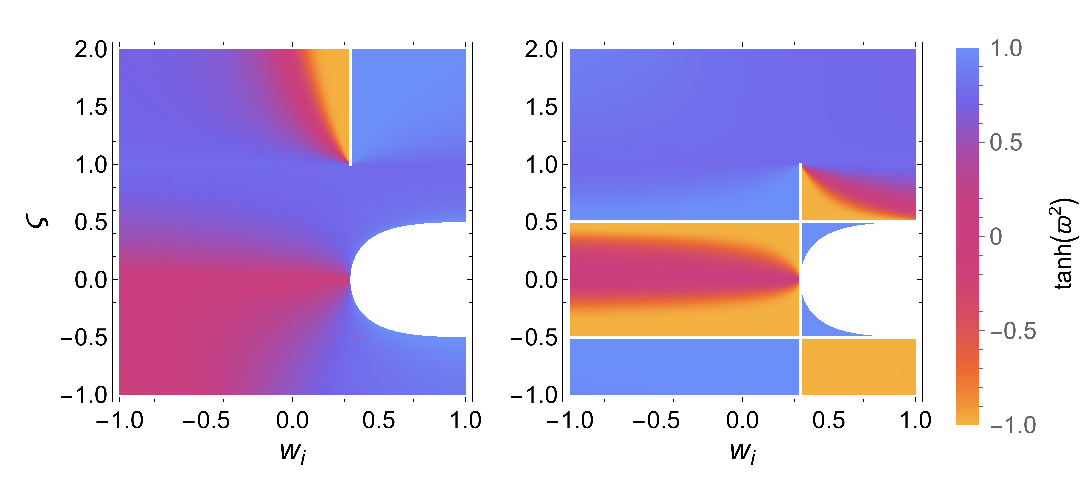
\includegraphics[width=\textwidth]{wibranch.pdf}
  \caption{The two branches of \cref{eq:stigma-cpr-branches} for the fixed-point value $\cpr_i$, over the plane of the equation of state parameter $w_i$ and the coupling $\varsigma$. The colour shows $\tanh(\cpr^2)$, which compresses the divergences near the poles into a finite range. White marks the region in which the term $2 - 6 w_i + (\varsigma + 3 w_i \varsigma)^2$ is negative and no real solution exists, together with the poles at $\varsigma = \pm 1/2$. The pole at $w_i = 1/3$ is examined more carefully in the text. This reproduces the fixed-point structure presented in~\citep{Barker:2020gcp}.}
  \label{fig:stigma-wibranch}
\end{figure*}
Considering the radiation-era fixed point directly and substituting $w_i = 1/3$ into the field equation that gave rise to~\cref{eq:stigma-cpr-eom} reduces it to
\begin{equation}
  \left.\frac{\partial L}{\partial \cpr}\right|_{\cpr=\cpr_i}^{w_i=1/3}
  \propto -\frac{(\cpr_i^2 - 1)(\varsigma-1)\cpr_i \varsigma }{(\cpr_i^2 - \varsigma)^2} = 0.
  \label{eq:inicondition}
\end{equation}
Ignoring the trivial solutions $\cpr_i=0$ and $\varsigma=0$, the numerator shows that the radiation-epoch fixed-point value can be obtained from either $\cpr_i^2=1$ or $\varsigma=1$. Since the purpose of this study is to explore the departure of TorC from \LCDM{} in the late Universe through varying $\varsigma$, $\cpr_i^2=1$ is adopted as the initial condition for $\varpi$. Further discussion is given in~\cref{app:stigma-power}. 

\paragraph*{Choice of parameter range}The above discussion assumes $\lambda=0$. For $\lambda\neq0$, applying the same procedure gives a time-dependent solution for $\cpr_i$. Nevertheless, in the early-time limit $t\to0$, $\cpr_i^2\to1$ still holds. Moreover, a general initial value~$\cprr$ can be allowed for~$\varpi$. The generic power series is then found by setting $a(\tau) = \sum_{n=1}^{\infty} a_n \tau^n$ and $\cpr(\tau) = \cprr + \sum_{n=1}^{\infty} c_n \tau^n$ and substituting these expressions into the equations of motion in conformal time, using the equation for $a'(\tau)$ obtained from~\cref{eq:stigma-F1} together with the equation for $\cpr''(\tau)$ obtained from a combination of~\cref{eq:stigma-F2,eq:stigma-cpr-eom}. The coefficients $a_n$ and $c_n$ are then solved order by order in $\tau$; at lowest order this gives
\begin{align}
		& \frac{(\varsigma -1) \varsigma \cprr (\cprr^2 - 1)((5 - 8 \varsigma)\varsigma + (4\varsigma^2 - 1)\cprr^2 )}{(4\varsigma^2- 1)(\varsigma - \cprr^2)^2} = 0, \\
		& a_1 = \pm \frac{2 H_0 \sqrt{\Omega_{\mathrm{r}}\varsigma(\cprr^2-\varsigma)}}{\abs{\cprr} \sqrt{\upsilon_2((5 - 8 \varsigma)\varsigma + (4\varsigma^2 - 1)\cprr^2 )}}. \label{eq:signofa1}
\end{align}
For $\varsigma\neq1$, solving these equations simultaneously and requiring a real, expanding solution with $a_1>0$ separates the allowed solutions into positive and negative branches:
\begin{alignat}{2}
		\boxed{+} \; \cprr &= \pm 1, \;\, & \varsigma &\in \bigl(-\infty,-\tfrac{1}{2}\bigr) \cup \bigl(-\tfrac{1}{2},0\bigr) \cup (1,\infty), \label{eq:posbranch}\\
\boxed{-} \; \cprr &= \pm 1, \;\, & \varsigma &\in \bigl(\tfrac{1}{4},\tfrac{1}{2}\bigr) \cup \bigl(\tfrac{1}{2},1\bigr). \label{eq:negbranch}
\end{alignat}
The negative-branch solutions encounter poles during their evolution due to factors of ($\varsigma-\varpi^2$) in the denominators of the field equations and are therefore not considered further. The positive branch contains two disconnected regions, $\varsigma<0$ and $\varsigma>1$, for which the background evolution remains regular. In this paper, attention is restricted to $\varsigma > 1$, as this region is continuously connected to the \LCDM{} limit at $\varsigma = 1$, and therefore provides the natural extension of TorC. The $\varsigma<0$ region forms a disconnected branch of parameter space and is left for future investigation.

\subsection{Effect of the $\varsigma$TorC parameters on distances}
\label{sec:stigma-effects}
\paragraph*{Computing distances} The late-time expansion history predicted by $\varsigma$TorC is constrained using DESI DR2 baryon acoustic oscillation (BAO) data and Type Ia supernova distance measurements from Pantheon+, DES5Y, \CLAUD{DES-Dovekie,} and Union3. These observables can be constructed directly from the dimensionless expansion history $E(z)$, and therefore do not require the evolution of cosmological perturbations. The power series solutions in~\cref{eq:powa,eq:powcp}, together with the field equation~\cref{eq:stigma-F1}, reveal that $H_0$ and $\sqrt{\upsilon_2}$ enter the time evolution only through the combination $H_0/\sqrt{\upsilon_2}$. The rescaling $t\rightarrow (H_0/\sqrt{\upsilon_2})t$ therefore absorbs this combination into an overall normalisation of the background evolution. Since $E(z)$ is insensitive to this overall normalisation, $\upsilon_2$ does not affect the distance measurements considered here. The relevant theory parameters are therefore $\varsigma$, $\lambda$, and $\Omega_\Lambda$, together with the standard cosmological parameters $\Omega_\mathrm{m}$ and $H_0r_\mathrm{d}$. The relevant parameters are summarised in~\cref{tab:stigma-params}.
\begin{table}[t]
\centering
\begin{tabularx}{\columnwidth}{c|>{\raggedright\arraybackslash}X}
\toprule
$\varsigma$ & Ratio of the torsional couplings, restricted to $\varsigma>1$\\
$\lambda$ & Dimensionless torsional coupling\\
$\OL$ & Bare dark energy density parameter\\
\midrule
$\Om$ & Matter density parameter\\
$H_0 r_\mathrm{d}$ & Hubble constant times the sound horizon at the drag epoch\\
\bottomrule
\end{tabularx}
\caption{Parameters of $\varsigma$TorC relevant to the distance measurements considered in this paper. The top rows list the three additional parameters of $\varsigma$TorC, while the bottom rows list the standard \LCDM{} distance parameters constrained by DESI.}
\label{tab:stigma-params}
\end{table}
The effect of the parameters on the BAO distances is computed by solving the coupled ODEs in~\cref{eq:stigma-F1,eq:stigma-F2}. The resulting $E(z)$ is then used to compute the DESI DR2 BAO distance measures. \Cref{fig:stigma-rainbow-distances} follows the presentation of DESI~\citep{DESI:2024mwx}, using combinations of the BAO distance that reduce their overall redshift dependence and highlight the effect of varying each parameter. Parameters not varied in each panel are fixed to their GR correspondence values.

\paragraph*{Effect of the torsional coupling ratio} The dependence of the comoving Hubble horizon $H_0/(aH)$ on $\varsigma$ is shown in~\cref{fig:stigma-horizon-common}, with the change most significant during matter domination.
The inset shows the corresponding evolution of $\varpi^2$, which departs increasingly from unity at late times as $\varsigma$ is increased. In TorC with $\varsigma=1$, $\varpi^2$ instead approaches unity at late times. This suggests that, for $\varsigma\neq1$, the effects of $\lambda$ and $\Omega_\Lambda$ no longer reduce to the simple combined contribution $\OL+\lambda$ found for $\varsigma=1$. The $\varsigma$ and $\Omega_\mathrm{m}$ panels in~\cref{fig:stigma-rainbow-distances} show that increasing $\varsigma$ modifies the expansion history in a way similar to increasing $\Omega_\mathrm{m}$. A larger $\Omega_\mathrm{m}$ raises $E(z)$ during matter domination, reducing both $D_H$ and $D_M$, and hence $D_V$. Since $D_H$ depends directly on $E(z)$ at a given redshift, whereas $D_M$ depends on the integrated expansion history, $D_H$ decreases more strongly and $D_M/D_H$ increases. The same behaviour is seen for increasing $\varsigma$. This suggests that $\varsigma$ and $\Omega_\mathrm{m}$ may have similar effects on the distance measurements.

\begin{figure*}[tp]
\centering
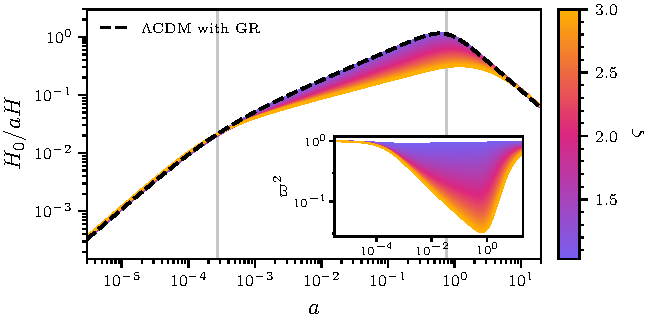
\includegraphics[width=0.8\textwidth]{hubble_horizon_varsigma_common.pdf}
\caption{Comoving Hubble horizon $H_0/(aH)$ as a function of the scale factor $a$, for values of $\varsigma$ spanning the range shown by the colour bar. The inset shows the corresponding evolution of $\varpi^2$. The dashed curve shows the \LCDM{} prediction in GR. The three grey vertical lines separate the radiation-, matter-, and dark-energy-dominated epochs, showing that the effect of $\varsigma$ is most significant during the matter-dominated epoch.}
\label{fig:stigma-horizon-common}
\end{figure*}

\begin{figure*}[tp]
\centering
\begin{subfigure}{0.49\linewidth}
\centering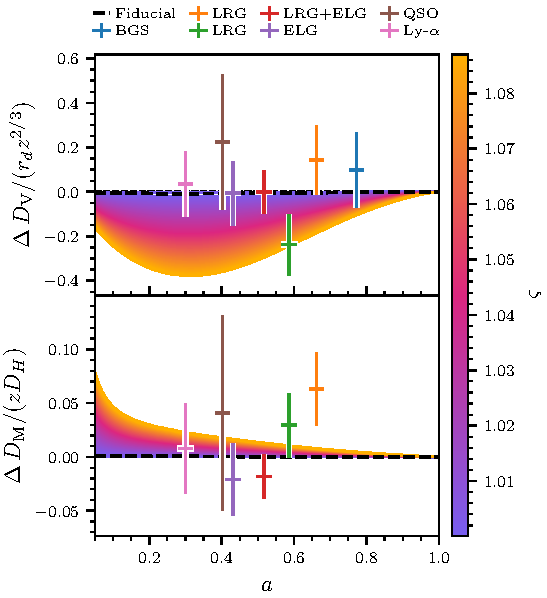
\includegraphics[width=\linewidth]{TorC_rainbow_lam_stigma.pdf}
\end{subfigure}
\hfill
\begin{subfigure}{0.49\linewidth}
\centering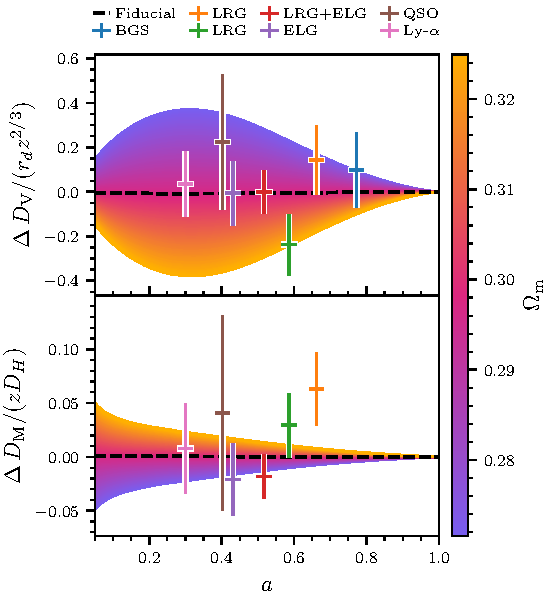
\includegraphics[width=\linewidth]{TorC_rainbow_lam_omega_m.pdf}
\end{subfigure}

\vspace{\baselineskip}
\begin{subfigure}{0.49\linewidth}
\centering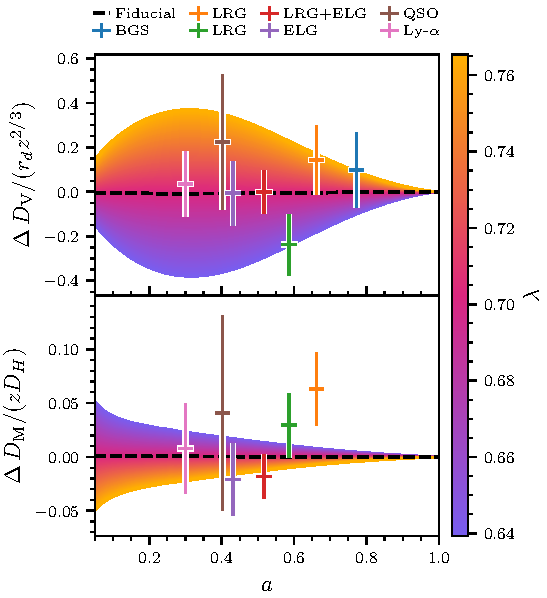
\includegraphics[width=\linewidth]{TorC_rainbow_lam_lam.pdf}
\end{subfigure}
\hfill
\begin{subfigure}{0.49\linewidth}
\centering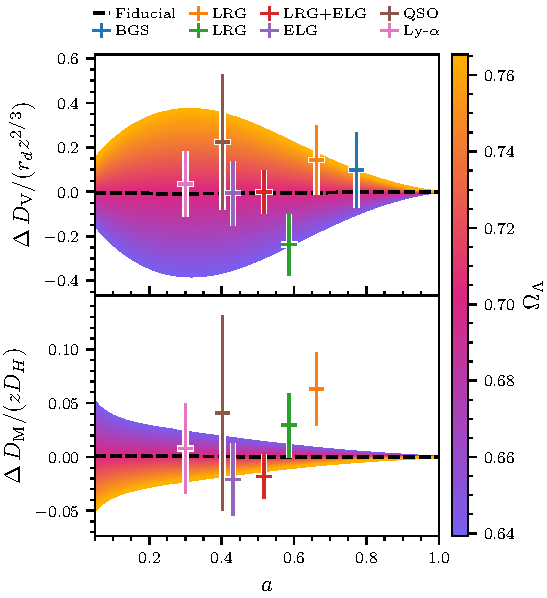
\includegraphics[width=\linewidth]{TorC_rainbow_lam_OmL.pdf}
\end{subfigure}
\caption{Effect of the $\varsigma$TorC parameters on the DESI DR2 distance observables. The plotting convention follows~\citep{DESI:2024mwx}, with the panels showing differences relative to the fiducial \LCDM{} case (dashed) in $\Delta D_\mathrm{V}/(r_\mathrm{d} z^{2/3})$ (upper sub-panel) and $\Delta D_\mathrm{M}/(z D_\mathrm{H})$ (lower sub-panel) as a function of the scale factor $a$. The colour bar indicates the range of the varied parameter: $\varsigma$ and $\Om$ in the top row, and $\lambda$ and $\OL$ in the bottom row. The remaining parameters are fixed to their fiducial values to isolate the effect of each parameter. The DESI DR2 BAO measurements for the BGS, LRG, LRG+ELG, ELG, QSO and Ly$\alpha$ tracers are overplotted with their uncertainties. Note that the $\lambda$ panel should be interpreted with some care, since the effect of $\lambda$ also depends on $\varsigma$, which is fixed to its fiducial value in this figure.}
\label{fig:stigma-rainbow-distances}
\end{figure*}

\paragraph*{Effect of bare dark energy density and torsional coupling} The bottom row of~\cref{fig:stigma-rainbow-distances} shows that $\lambda$ and $\Omega_\Lambda$ produce very similar changes in the BAO distances. Since the expansion history is normalised, increasing $\Omega_\Lambda$ increases the late-time expansion relative to earlier times, giving a smaller $E(a)$ for $a<1$. This increases both $D_H$ and $D_M$, and hence increases $D_V$ while decreasing $D_M/D_H$. Increasing $\lambda$ produces the same behaviour. Both parameters therefore affect the BAO distances in the opposite direction to increasing $\Omega_\mathrm{m}$. However, this comparison should be interpreted with some care, since the remaining parameters are fixed to their fiducial values. In particular, $\varsigma$ is fixed close to unity, whereas the effect of $\lambda$ depends on $\varsigma$. In~\cref{eq:stigma-F1,eq:stigma-F2}, $\lambda$ couples to $\varpi^2$, whose evolution changes with $\varsigma$ as shown in the inset of~\cref{fig:stigma-horizon-common}. The effect of $\lambda$ will therefore deviate more strongly from that of $\Omega_\Lambda$ as $\varsigma$ increases.

\section{Method}
\label{sec:stigma-method}
The $\varsigma$TorC model is compared with \LCDM{} and the CPL model using DESI DR2 distance measurements, both alone and in separate combinations with Pantheon+, DES5Y, \CLAUD{DES-Dovekie,} and Union3. Three $\varsigma$TorC cases are considered: a $\lambda$-only model, an $\Omega_\Lambda$-only model, and a model in which both $\lambda$ and $\Omega_\Lambda$ are varied. The priors adopted for each model are summarised in~\cref{tab:stigma-priors}.

\subsection{Numerical implementation}
The background evolution is obtained by integrating the coupled equations in~\cref{eq:stigma-F1,eq:stigma-F2} using \texttt{Julia}~\citep{bezanson2015juliafreshapproachnumerical}.\footnote{The background solver is implemented in \texttt{Julia}, which gave the best performance among the numerical implementations benchmarked for this analysis, making the full analysis possible to run on a local laptop.} The resulting solution is used to construct the dimensionless expansion history $E(z)$ and the corresponding DESI DR2 BAO, Pantheon+, DES5Y, \CLAUD{DES-Dovekie,} and Union3 distance observables. The priors, likelihoods, and nested-sampling pipeline are implemented in \texttt{JAX}~\citep{jax2018github}, with the Julia background solver called during the sampling.\footnote{Because the late-time analysis needs only the background expansion, no Boltzmann code is required, and each likelihood evaluation reduces to solving the stiff ODE system of~\cref{eq:stigma-F1,eq:stigma-F2}. \texttt{Julia} offers mature, fast solvers for such systems. \texttt{BlackJAX} implements nested slice sampling in \texttt{JAX}, which evaluates many live points in parallel on vectorised hardware, making it well suited to the large number of model and data combinations considered here.} Posterior distributions and Bayesian evidences are obtained using the nested slice sampling algorithm implemented in \texttt{BlackJAX}~\citep{Yallup:2026nested} with 1000 live points.

\subsection{Priors}
\begin{table}[t]
\centering
\begin{tabular}{c|c}
\toprule
Parameter & Prior \\
\midrule
$H_0 r_\mathrm{d}$ & $\left[3650, 18250 \right]$~km\,s$^{-1}$ \\
$\Omega_\mathrm{m}$ & $\left[0.01, 0.99\right]$\\
\midrule
$\varsigma$ & $2/(1+\varsigma)^{2}$\\
$\Omega_\Lambda$ & \CLAUD{$\left[0.0, 1.5\right]$}\\
$\lambda$ & $\left[0.0, 1.5\right]$\\
\midrule
$w_0$ & $\left[-3, 1\right]$ \\
$w_a$ & $\left[-3, 2\right]$ \\
\bottomrule
\end{tabular}
\caption{Priors used for the parameters in \LCDM{}, $\varsigma$TorC, and CPL models. The priors are uniform within the range, except for $\varsigma$ which has a power-law prior with a lower bound of $\varsigma = 1.0001$. For the CPL model, the additional constraint $w_0+w_a<0$ is imposed to ensure matter domination at high redshift.}
\label{tab:stigma-priors}
\end{table}
The priors used for the parameters in the $\varsigma$TorC, \LCDM{}, and CPL models are summarised in~\cref{tab:stigma-priors}. Most of the priors are uniform over the ranges indicated in the table. For the CPL model, an additional prior,
\begin{equation}
		w_0 + w_a < 0,
\end{equation}
is imposed following the DESI analysis, to enforce a period of high-redshift matter domination. Since $\varsigma$ is defined as the ratio of the two negative couplings, $\varsigma=\sigma_1/\sigma_2$ as in~\cite{Barker:2020elg}, its prior is constructed from exponential priors on their magnitudes, $|\sigma_1|$ and $|\sigma_2|$. Defining $x=|\sigma_1|$ and $y=|\sigma_2|$, with $\varsigma=x/y$, and transforming from $(x,y)$ to $(\varsigma,y)$ using $x=\varsigma y$, marginalisation over $y$ gives the power-law prior, $\pi(\varsigma) \propto (1+\varsigma)^{-2}$. For the branch investigated in this paper, $\varsigma>1$, the prior is normalised as
\begin{equation}
		    \pi(\varsigma)=\frac{2}{(1+\varsigma)^2}, \qquad \varsigma>1.
\end{equation}
The lower bound $\varsigma=1.0001$ is imposed to remain within the $\varsigma>1$ branch and avoid the pole at $\varsigma=1$.

\subsection{Bayesian model comparison}
\label{sec:model-comparison}
The Bayesian evidence $\mathcal{Z}$ of a model can be decomposed into the posterior-weighted log likelihood,
\begin{equation}
		\langle \log \mathcal{L}(\theta) \rangle_\mathcal{P} = \int \log \mathcal{L}(\theta) P(\theta | D) \mathrm{d}\theta,
\end{equation}
where~$P(\theta | D)$ is the posterior distribution of the parameters given the data~$D$, and the Kullback--Leibler (KL) divergence~\citep{Handley:2019pqx, Kullback:1951zyt}
\begin{equation}
		\mathcal{D}_{\mathrm{KL}} = \int P(\theta | D) \log \frac{P(\theta | D)}{\pi(\theta)} \mathrm{d}\theta,
\end{equation}
which quantifies how much the posterior distribution has contracted relative to the prior. The first term measures how well the model fits the data, averaged over the posterior. The second acts as a complexity penalty --- a model with a large parameter space that is significantly narrowed by the data will have a larger value of~$\mathcal{D}_{\mathrm{KL}}$. We also report the maximum log likelihood,~$\log \mathcal{L}_\mathrm{max}$, which measures the best fit a model can achieve irrespective of its complexity. For models~$M_1$ and~$M_2$ with uniform prior model probabilities, the ratio of posterior probabilities gives the Bayes factor $\mathcal{Z}_1 / \mathcal{Z}_2$. In logarithmic form,
\begin{equation}
		\begin{split}
				\Delta \log \mathcal{Z} & = \log \mathcal{Z}_1 - \log \mathcal{Z}_2\\
										& = \Delta \langle \log \mathcal{L}(\theta) \rangle_\mathcal{P} - \Delta \mathcal{D}_{\mathrm{KL}},
		\end{split}
		\label{eq:BayesFactor}
\end{equation}
where values of~$\Delta \log \mathcal{Z} > 0$ indicate that $M_1$ is supported over $M_2$ by a factor of $\exp(\Delta \log \mathcal{Z})$. This decomposition allows the source of model preference to be identified, comparing the goodness-of-fit and the complexity penalty of the models.

\section{Results}
\label{sec:stigma-results}
The constraints on $\varsigma$TorC are presented in this section and compared with those obtained for \LCDM{} and CPL. DESI DR2 BAO data are first considered alone to examine how the additional $\varsigma$TorC parameters are constrained by the distance measurements. Pantheon+, DES5Y, \CLAUD{DES-Dovekie,} and Union3 are then added separately to assess how the supernova datasets modify these constraints. Finally, the overall viability of $\varsigma$TorC, \LCDM{}, and CPL models is quantified using the Bayesian evidence.

\subsection{Constraints from DESI DR2 BAO}
\begin{figure*}[tp]
\centering
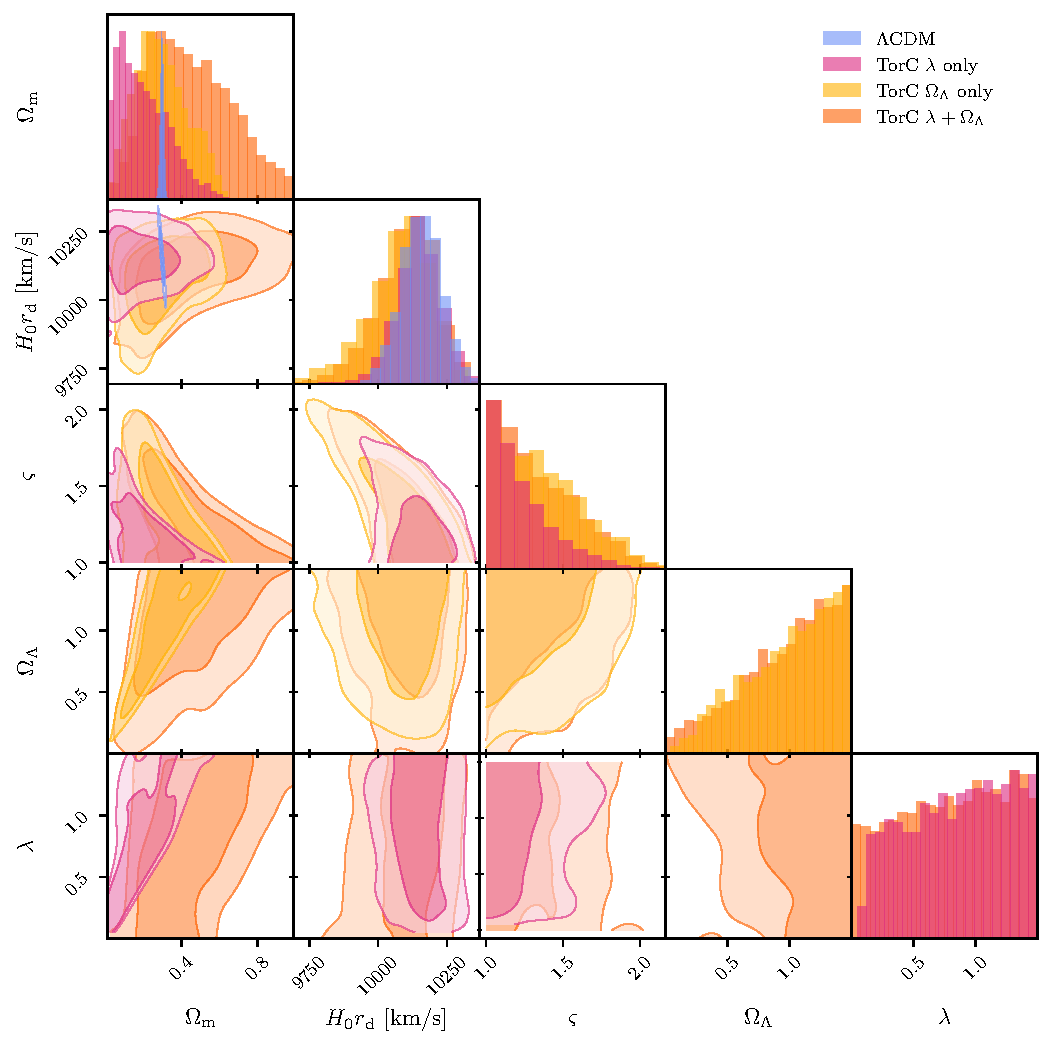
\includegraphics[width=0.85\textwidth]{corner_torc_lcdm_bao.pdf}
\caption{Posterior distributions for \LCDM{} (blue) and the three $\varsigma$TorC cases constrained by DESI DR2 BAO distance measurements: the $\lambda$-only model (pink), the $\Omega_\Lambda$-only model (yellow), and the joint $\lambda+\Omega_\Lambda$ model (orange). Each was run with \texttt{BlackJAX} nested sampling using the DESI DR2 BAO likelihood, with the settings in~\cref{sec:stigma-method}. The posterior plot is created with \anesthetic{}~\citep{Handley:2019mfs}.}
\label{fig:torc-lcdm-bao-corner}
\end{figure*}

\paragraph*{Parameter constraints} The posterior distributions of the $\varsigma$TorC and \LCDM{} parameters constrained by DESI DR2 BAO distances are shown in~\cref{fig:torc-lcdm-bao-corner}. The additional freedom in $\varsigma$TorC broadens the constraint on $\Omega_\mathrm{m}$ relative to \LCDM{}. A correlation between $\varsigma$ and $\Omega_\mathrm{m}$ is also visible, consistent with their similar effects on the BAO distances discussed in~\cref{sec:stigma-effects}. Unlike in the $\varsigma=1$ case, where the late-time expansion depends only on $\OL+\lambda$~\cite{Legner:2026}, the $\lambda$--$\Omega_\Lambda$ plane does not exhibit a strong degeneracy, with the joint posterior allowing a broader range of combinations. This is consistent with the additional correlation between $\lambda$ and $\varsigma$, since the effect of $\lambda$ depends on the evolution of $\varpi^2$, which itself varies with $\varsigma$, as discussed in~\cref{sec:stigma-effects}. Both $\lambda$ and $\Omega_\Lambda$ are also correlated with $\Omega_\mathrm{m}$, consistent with their opposite effects on the BAO distances to that of increasing $\Omega_\mathrm{m}$. The CPL model is omitted from this figure for clarity; its constraints in the $H_0r_\mathrm{d}$--$\Omega_\mathrm{m}$ plane are presented in~\cref{fig:stigma-grid-om-h0rd}.


\begin{figure*}[tp]
\centering
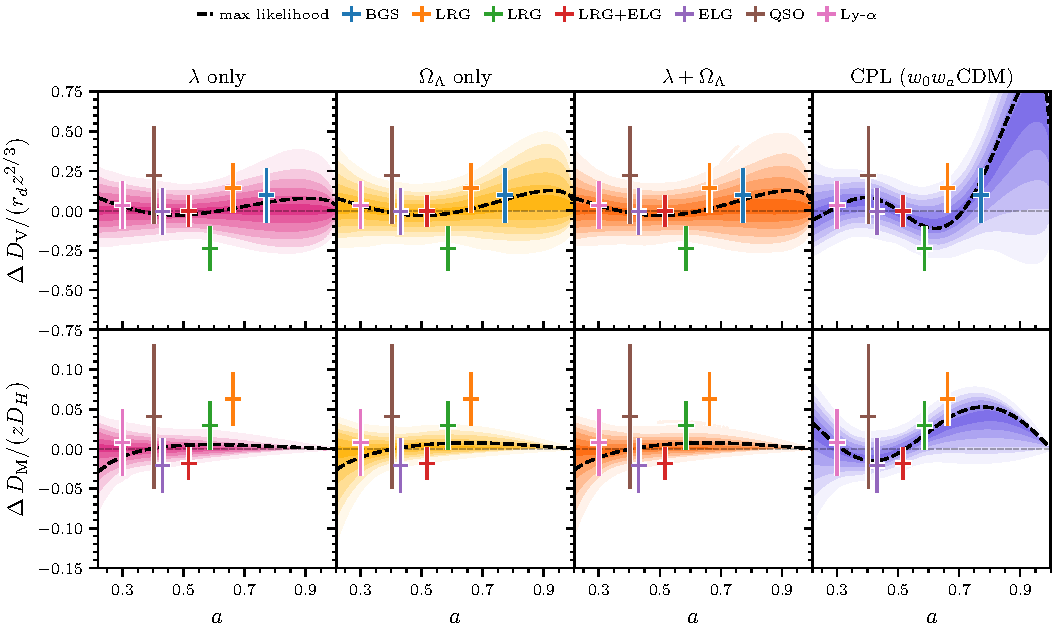
\includegraphics[width=\textwidth]{fgivenx_models.pdf}
\caption{Posterior predictions for the DESI DR2 BAO distances in the $\varsigma$TorC and CPL models. The upper panels show $\Delta D_\mathrm{V}/(r_\mathrm{d} z^{2/3})$, while the lower panels show $\Delta D_\mathrm{M}/(z D_\mathrm{H})$, with both quantities defined relative to the \LCDM{} best-fit prediction. The posterior contours are shown at intervals of $0.5\sigma$. The dashed curves indicate the maximum-likelihood predictions, with the DESI DR2 measurements overlaid. The four models shown are the $\lambda$-only, $\OL$-only, $\lambda+\OL$, and CPL ($w_0w_a$CDM) models. Generated using \texttt{fgivenx}~\citep{fgivenx}.}
\label{fig:stigma-fgivenx-models}
\end{figure*}

\paragraph*{BAO distance reconstruction} The posterior predictions for the DESI DR2 BAO observables in the $\varsigma$TorC and CPL models are shown in~\cref{fig:stigma-fgivenx-models}. The distances are plotted relative to the \LCDM{} best-fit prediction, such that zero corresponds to \LCDM{}. The dashed curves indicate the maximum-likelihood solution for each model. The three $\varsigma$TorC cases produce similar modifications to the BAO distances, whereas the CPL model in the right-most panel allows a stronger redshift dependence. This shows that although both extensions can depart from the \LCDM{} prediction while fitting the DESI BAO measurements, they modify the distance observables in different ways.

\subsection{Constraints with supernova data}
\begin{figure*}[tp]
\centering
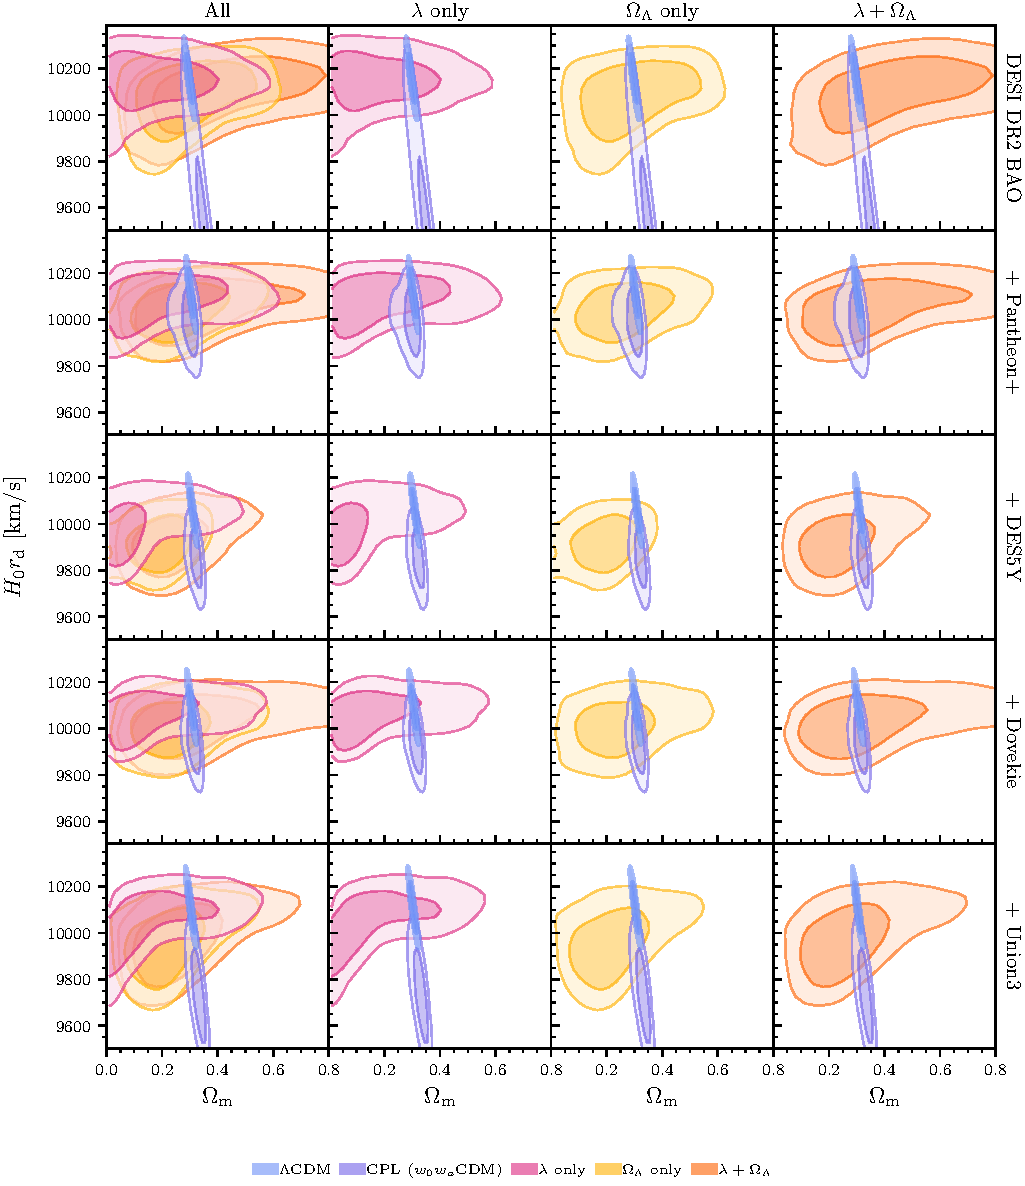
\includegraphics[width=\textwidth]{grid_om_h0rd.pdf}
\caption{Posterior distributions in the $\Om$--$H_0 r_\mathrm{d}$ plane, showing all five models --- \LCDM{} (blue), CPL (purple), $\lambda$-only (pink), $\Omega_\Lambda$-only (yellow), and combined $\lambda$ and $\Omega_\Lambda$ (orange) $\varsigma$TorC models. For $\varsigma$TorC models, the columns show all three models, then $\lambda$ only, $\OL$ only, and $\lambda + \OL$ in turn. \LCDM{} and CPL posteriors are shown in all panels for comparison. The rows show, from top to bottom, DESI DR2 BAO alone and DESI DR2 BAO combined separately with Pantheon+, DES5Y, \protect\CLAUD{DES-Dovekie,} and Union3.}
\label{fig:stigma-grid-om-h0rd}
\end{figure*}

Type Ia supernova data are included separately in combination with DESI DR2 BAO, with the resulting constraints in the $H_0r_\mathrm{d}$--$\Omega_\mathrm{m}$ plane shown in~\cref{fig:stigma-grid-om-h0rd}. For DESI DR2 BAO alone, the $\varsigma$TorC models broaden the posterior distribution of $\Omega_\mathrm{m}$ relative to \LCDM{}, while CPL broadens the constraint on $H_0r_\mathrm{d}$. Adding supernova data tightens the CPL contours. The $\lambda$-only $\varsigma$TorC model behaves differently from the other cases, favouring lower values of $\Omega_\mathrm{m}$, particularly when DES5Y is included. This behaviour could arise from the coupled dependence of the expansion history on $\Omega_\mathrm{m}$, $\varsigma$, and $\lambda$. As discussed in~\cref{sec:stigma-effects}, $\varsigma$ modifies the expansion during matter domination while also changing the evolution of $\varpi^2$, and hence the contribution of the $\lambda$ term. Their interplay therefore produces a different $\Omega_\mathrm{m}$--$\varsigma$ correlation from that of the $\Omega_\Lambda$-only case. The corresponding posterior distributions in the $\varsigma$--$\Omega_\mathrm{m}$ plane are shown in~\cref{fig:stigma-grid-om-stigma} for each data combination.

\subsection{Model comparison}
\begin{figure*}[tp]
\centering
\begin{subfigure}{0.45\linewidth}
\centering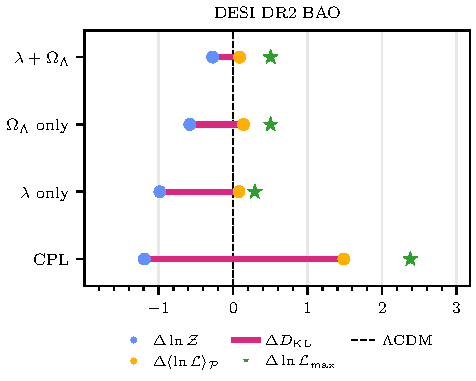
\includegraphics[width=\linewidth]{evidence_scatter_delta_bao.pdf}
\end{subfigure}
\hfill
\begin{subfigure}{0.45\linewidth}
\centering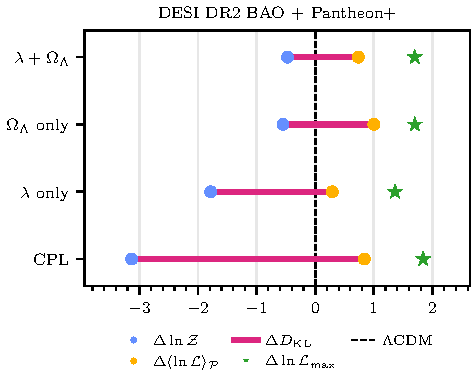
\includegraphics[width=\linewidth]{evidence_scatter_delta_bao_pp.pdf}
\end{subfigure}

\vspace{\baselineskip}
\begin{subfigure}{0.45\linewidth}
\centering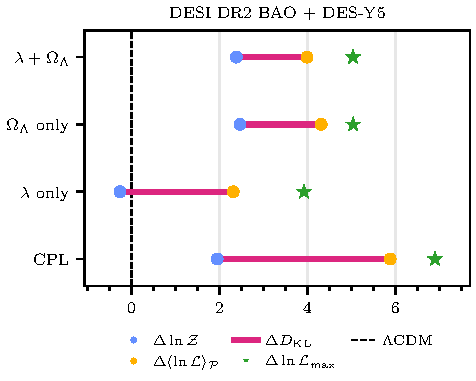
\includegraphics[width=\linewidth]{evidence_scatter_delta_bao_desy5.pdf}
\end{subfigure}
\hfill
\begin{subfigure}{0.45\linewidth}
\centering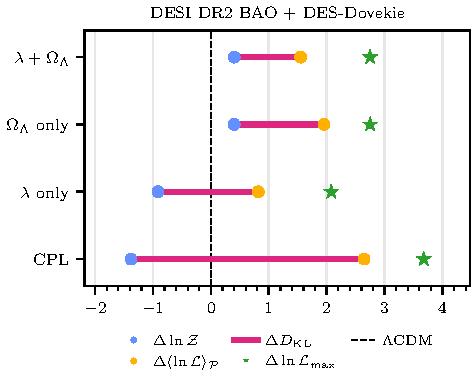
\includegraphics[width=\linewidth]{evidence_scatter_delta_bao_dov.pdf}
\end{subfigure}

\vspace{\baselineskip}
\begin{subfigure}{0.45\linewidth}
\centering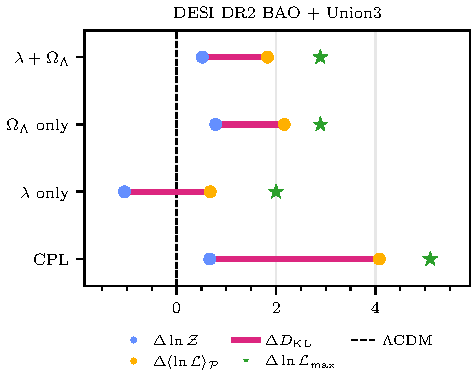
\includegraphics[width=\linewidth]{evidence_scatter_delta_bao_u3.pdf}
\end{subfigure}
\caption{Model comparison with Bayesian evidence relative to \LCDM{} for the $\varsigma$TorC and CPL models, showing the differences in log evidence in blue, posterior-averaged log likelihood in yellow, their difference showing the KL divergence in pink, and the maximum log likelihood in green. The datasets are DESI DR2 BAO alone (top left), with Pantheon+ (top right), \protect\CLAUD{with DES5Y (middle left), with DES-Dovekie (middle right), and with Union3 (bottom).}}
\label{fig:stigma-evidence-scatter}
\end{figure*}

\paragraph*{DESI-only} Model comparison is performed using the Bayesian evidence, with the results shown in~\cref{fig:stigma-evidence-scatter}. The figure shows differences relative to \LCDM{} in the log evidence, posterior-averaged log likelihood, KL divergence, and maximum log likelihood. For DESI DR2 BAO alone and in combination with Pantheon+, the $\varsigma$TorC models containing $\Omega_\Lambda$ have evidences comparable to \LCDM{} and are favoured over CPL. Although CPL reaches the highest maximum likelihood, its larger KL divergence results in a stronger complexity penalty. In contrast, despite the larger parameter space of $\varsigma$TorC, the corresponding complexity penalty remains relatively small. Since the KL divergence measures the information gained from the prior to the posterior, the weak constraints on the additional $\varsigma$TorC parameters lead to only a modest increase in $\mathcal D_{\mathrm{KL}}$.

\paragraph*{With supernovae data} A different behaviour is seen when DES5Y is included. The $\Omega_\Lambda$-only and $\lambda+\Omega_\Lambda$ $\varsigma$TorC models give log-evidence differences of \CLAUD{$\Delta\ln\mathcal{Z}_{\Omega_\Lambda}=2.468\pm0.138$ and $\Delta\ln\mathcal{Z}_{\lambda+\Omega_\Lambda}=2.382\pm0.141$}, respectively, indicating a moderate preference over \LCDM{}. Replacing DES5Y with DES-Dovekie removes this preference, giving \CLAUD{$\Delta\ln\mathcal{Z}_{\Omega_\Lambda}=0.40\pm0.14$ and $\Delta\ln\mathcal{Z}_{\lambda+\Omega_\Lambda}=0.40\pm0.14$}, comparable to \LCDM{}. The replacement also removes the preference of CPL from $\Delta\ln\mathcal{Z}=1.95\pm0.15$ to $\Delta\ln\mathcal{Z}=-1.39\pm0.15$. For Union3, the $\varsigma$TorC models have evidences comparable to \LCDM{}. The $\lambda$-only $\varsigma$TorC model is consistently less favoured than the other $\varsigma$TorC cases across all data combinations, suggesting that the data do not favour replacing the bare dark energy contribution $\Omega_\Lambda$ entirely with the torsional coupling~$\lambda$.

\section{Conclusions}
\label{sec:stigma-conclusion}
\paragraph*{Summary} In this paper, the extended $\varsigma$TorC model is explored, in which $\varsigma=\sigma_1/\sigma_2$ is allowed to vary. Since TorC approaches the \LCDM{} background at late times, limiting the ability of late-time probes to distinguish the two models, relaxing $\sigma_1=\sigma_2$ gives the theory additional freedom in its late-time expansion. From the early-time analysis, it was found that allowing $\varsigma$ to vary fixes the initial torsion scalar field to $\cprr^2=1$. Thus, $\varsigma$ and the initial value $\cprr$ used as a free parameter in previous work~\citep{Legner:2025hrt} cannot both be varied independently. Varying $\varsigma$ also changes the evolution of the torsion field and hence the contribution of $\lambda$, motivating a new comparison of the $\lambda$-only, $\Omega_\Lambda$-only, and joint cases. The resulting cosmological evolution and the effects of $\varsigma$, $\lambda$, and $\Omega_\Lambda$ on the late-time distance observables used in the DESI BAO measurements are then explored.

\paragraph*{Cosmological constraints} The cosmological constraints were obtained from DESI DR2 BAO measurements, both alone and separately in combination with Pantheon+, DES5Y, \CLAUD{DES-Dovekie,} and Union3 supernova data. The posterior distributions show that the additional $\varsigma$TorC parameters broaden the allowed range of $\Omega_\mathrm{m}$ relative to \LCDM{}. The $\lambda$-only model shows a stronger tendency towards lower values of $\Omega_\mathrm{m}$, particularly for DES5Y. This behaviour arises from the joint dependence of $\Omega_\mathrm{m}$, $\varsigma$, and $\lambda$, since $\varsigma$ affects both the matter-era expansion and the evolution of $\varpi^2$, which is coupled with $\lambda$ in the field equations.

\paragraph*{Model comparison} The Bayesian model comparison shows that the $\varsigma$TorC models containing $\Omega_\Lambda$ have evidences comparable to \LCDM{} for DESI DR2 BAO alone and when combined with Pantheon+\CLAUD{, DES-Dovekie,} and Union3, while the combination with DES5Y gives a moderate preference over \LCDM{}. The $\lambda$-only model is consistently less favoured than the other $\varsigma$TorC models, suggesting that removing the bare dark energy contribution and relying on the $\lambda$ term alone is not preferred by the data. Although the $\varsigma$TorC models contain additional parameter space relative to \LCDM{} due to their additional parameters $\varsigma$, $\lambda$, and $\Omega_\Lambda$, this does not result in a larger complexity penalty. This is because the additional parameters remain weakly constrained by the data and therefore lead to a smaller information gain. This is in contrast to CPL, which can achieve a higher maximum likelihood but has a larger KL divergence, resulting in a lower Bayesian evidence in comparison with $\varsigma$TorC. The contribution of this analysis to the dynamical dark energy debate is therefore that this gravitationally motivated modification of the late-time expansion is at least as competitive as the phenomenological CPL model once the Occam penalty is included, being moderately preferred over \LCDM{} with DES5Y (\CLAUD{$\Delta\ln\mathcal{Z}=2.47\pm0.14$ and $2.38\pm0.14$} for the $\OL$-only and joint $\lambda+\OL$ models). DES-Dovekie was also tested, since it has been linked to a tension between DES5Y and DESI DR2 within \LCDM{}~\citep{Ong:2025utx,Ong:2026tta}. With DES-Dovekie, the preference for CPL over \LCDM{} is removed ($\Delta\ln\mathcal{Z}=-1.39\pm0.15$, compared with $1.95\pm0.15$ for DES5Y), while the $\varsigma$TorC models containing $\Omega_\Lambda$ remain comparable to \LCDM{} (\CLAUD{$\Delta\ln\mathcal{Z}=0.40\pm0.14$ and $0.40\pm0.14$}).

\paragraph*{Implications for $\varsigma$TorC} An important aspect of this work is that the late-time distance measurements provide a direct test of the background cosmology of an underlying theory of gravity without requiring the evolution of cosmological perturbations. Unlike phenomenological extensions such as CPL, the modified expansion history in $\varsigma$TorC follows directly from the theory's field equations. DESI BAO and supernova measurements can therefore be used to test the theory consistently at the background level using distance data alone. The fact that $\varsigma$TorC remains statistically competitive with \LCDM{}, \CLAUD{and is preferred with DES5Y but not with its DES-Dovekie reanalysis}, shows that a gravity-motivated modification of the late-time expansion can be consistent with current distance measurements without introducing a phenomenological parametrisation of the expansion history.
\paragraph*{Future work} The same distance-based approach could be used to test directly the curvature-screening property of TorC. As discussed in~\cite{Barker:2020elg}, the condition $\sigma_3=0$ screens TorC from spatial curvature, removing the contribution of $\Omega_k$ from the background expansion~\citep{Barker:2020gcp}, while its geometrical contribution to the distances remains. In a spatially curved Universe, the transverse comoving distance $D_M$ depends on curvature both explicitly, through the geometric relation between radial and transverse comoving distances, and implicitly, through the integral of $1/E(z)$ in~\cref{eq:transdistance}. Curvature screening removes the implicit dependence while leaving the explicit one unchanged. DESI BAO measurements are particularly suited to separating these effects, since $D_H(z)$ probes the expansion history directly, whereas $D_M(z)$ is sensitive to both the integrated expansion history and the spatial geometry. Combining these measurements with Type Ia supernova distances would therefore provide a direct late-time test of curvature screening in TorC and, provided the screening persists for $\varsigma\neq1$, in $\varsigma$TorC, again without requiring a cosmological perturbation theory. A related question concerns light propagation. This analysis assumes that photons follow the null geodesics of the metric, as in GR, so that spatial curvature affects cosmological distances through the usual geometric relation. In the presence of torsion, however, the propagation of light can in principle depend on how it couples to the torsionful connection, potentially modifying the optical effects associated with spatial curvature. These effects would need to be understood before curvature-screening constraints from distance measurements could be interpreted with full confidence. The disconnected $\varsigma<0$ branch of the background solutions also remains to be explored. More broadly, the numerical and statistical tools developed here are not specific to TorC: the same background-only pipeline can be applied to other extended theories of gravity, providing a bridge between theoretically motivated modifications of gravity and their observational constraints from late-time distance data.

\begin{acknowledgments}
\CLAUD{The authors would like to thank Adam Ormondroyd for his code base, on which this work is based~\citep{Ormondroyd:2025iaf}. The authors acknowledge the use of \texttt{NumPy}~\citep{harris2020array}, \texttt{SciPy}~\citep{2020SciPy-NMeth}, \texttt{JAX}~\citep{jax2018github}, \texttt{Julia}~\citep{bezanson2015juliafreshapproachnumerical}, \texttt{BlackJAX}~\citep{Yallup:2026nested}, \texttt{anesthetic}~\citep{Handley:2019mfs}, and \texttt{Matplotlib}~\citep{Hunter:2007} for numerical computations, sampling, and plotting.}
\paragraph*{\CLAUD{Generative AI declaration}} \CLAUD{Generative AI tools, namely Claude (Opus~5 and Opus~5.5, used through Claude Code), were used during the preparation of this paper as assistive tools. Their use included improving grammar and clarity with LaTeX, supporting coding and debugging, and assisting in the production of figures. The scientific content, methodology, interpretation of results, and conclusions presented in this paper remain those of the authors. }

\end{acknowledgments}

\bibliography{refs_notinspire,refs_torc,references}

\appendix

\section{Early-time power series}
\label{app:stigma-power}
Starting from the lowest-order conditions derived in~\cref{sec:stigma-cosmology}, which require $\varpi_r^2=1$ when $\varsigma$ is allowed to vary, we take $\varpi_r=1$ as the initial condition for $\varpi$ and solve the power series to higher orders, giving
\begin{align}
  a = {}& \pm \sgn[\varsigma(\varsigma - 1)] \frac{2 H_0 \sqrt{\Omega_{\mathrm{r,0}} \varsigma}}{\sqrt{\upsilon_2 (1- 4 \varsigma)}}\tau - \frac{H_0^2 \Omega_\mathrm{m}}{4 \upsilon_2} \tau^2 \nonumber\\
	& \pm \frac{H_0^3 \Omega_{\mathrm{m, 0}}^2 \sqrt{\varsigma (4 \varsigma - 1)}(\varsigma(24 \varsigma + 5) -2)}{64(-\upsilon_2)^{3/2} \sqrt{\Omega_{\mathrm{r}}}\abs{\varsigma - 1}(8 \varsigma^2 + \varsigma -3)}\tau^3 \nonumber\\
	& + \frac{H_0^4 \Omega_\mathrm{m,0}^3 (4 \varsigma - 1)}{512 \upsilon_2^2 \Omega_\mathrm{r,0} (\varsigma - 1)^2} \tau^4 \nonumber\\
	& \times \frac{240\varsigma^5-1510\varsigma^4-246\varsigma^3+357\varsigma^2+31\varsigma-6}{(8 \varsigma^2 + \varsigma -3)(20 \varsigma^2 + \varsigma -6)} \nonumber\\
	& + \mathcal{O}(\tau^5), \label{eq:powa}\\
\cpr = {}& 1 \mp \sgn[(\varsigma-1)(4\varsigma - 1)]\frac{H_0 \Omega_{\mathrm{m, 0}}\sqrt{4 \varsigma - 1}}{8 \sqrt{- \upsilon_2 \Omega_{\mathrm{r, 0}} \varsigma}} \tau \nonumber\\
	& - \frac{3 H_0^2 \Omega_{\mathrm{m, 0}}^2 (4 \varsigma - 1)(2 + \varsigma(3 \varsigma - 2))}{128 \upsilon_2 \Omega_{\mathrm{r, 0}}(\varsigma - 1)\varsigma (8 \varsigma^2 + \varsigma -3)}\tau^2 \nonumber\\
	& \pm \sgn[(\varsigma-1)(4\varsigma - 1)]\frac{H_0^3\Omega_\mathrm{m, 0}^3}{1024(\varsigma-1)^2}\Big(\frac{4 \varsigma -1}{- \upsilon_2 \varsigma \Omega_\mathrm{r,0}}\Big)^{3/2} \nonumber\\
	& \times \frac{\tau^3}{(8 \varsigma^2 + \varsigma -3)(20 \varsigma^2 + \varsigma -6)} \Big(192 \varsigma^6 + 380 \varsigma^5 \nonumber\\
	& -720 \varsigma^4 -225 \varsigma^3 +175 \varsigma^2 + 72 \varsigma - 36\Big) + \mathcal{O}(\tau^4). \label{eq:powcp}
\end{align}
For an expanding solution, the appropriate sign in the leading term of~\cref{eq:powa} is determined by the sign of $\varsigma(\varsigma-1)$, consistently with the branch conditions in~\cref{eq:posbranch,eq:negbranch}. The negative branch, corresponding to $0<\varsigma<1$ within the allowed intervals, encounters poles during its evolution due to the factors of $(\varsigma-\varpi^2)$ appearing in the field equations. The positive branch instead contains solutions with $\varsigma<0$ and $\varsigma>1$. In this paper, the analysis is restricted to the $\varsigma>1$ branch, since it is continuously connected to the GR-correspondence value $\varsigma=1$.

\section{Particle spectrum of $\varsigma$TorC}
\label{app:stigma-spectrum}
\CLAUD{The perturbation spectrum of $\varsigma$TorC around the non-zero torsion condensate is not derived in this paper and remains an area of active research. However, the particle spectrum around Minkowski spacetime with vanishing background torsion is well understood and provides the unitarity conditions used in~\cref{eq:stigma-conditions}. The particle spectrum describes the propagating degrees of freedom and their masses. The method used to obtain the spectrum is described in~\cref{app:spectrum-method}, and is applied to $\varsigma$TorC in~\cref{sec:stigma-spectrum}.}

\subsection{\texorpdfstring{\protect\CLAUD{Method}}{Method}}
\label{app:spectrum-method}
\CLAUD{The particle spectra are obtained with the spin-projection operator (SPO) algorithm as implemented in \psalter{}~\citep{Barker:2024juc,Barker:2025qmw}. Expanding a theory perturbatively to quadratic order about a vacuum gives a free-field approximation, whose propagator encodes which particle mode propagates, their masses, and whether their propagating mode is ghost free. The vacuum is a Minkowski spacetime with vanishing torsion. The particle spectra are computed in terms of the tetrad~$\tensor{e}{^a_\mu}$, its inverse~$\tensor{e}{_a^\mu}$ and the spin connection~$\tensor{\omega}{^{ab}_\mu}$, which are defined here as the input for \psalter{}. In the weak-field regime near Minkowski vacuum, the tetrad is expanded about the Kronecker delta as}
\begin{equation}
	\CLAUD{$\displaystyle \begin{gathered}\tensor{e}{_a^\mu}=\tensor*{\delta}{_a^\mu}+\tensor{f}{_a^\mu},\\ \tensor{e}{^a_\mu}=\tensor*{\delta}{^a_\mu}-\tensor{f}{_\mu^a}+\mathcal{O}(f^2).\end{gathered}$}
	\label{eq:pgt-perturbations}
\end{equation}
\CLAUD{The spin connection, $\tensor{\omega}{^{ab}_\mu}=\tensor{\omega}{^{[ab]}_\mu}$, is expanded about its vanishing Minkowski background value and is therefore itself treated as perturbatively small. At the lowest order of perturbation, the coordinate and the Lorentz indices can be related via the Kronecker delta, $\tensor*{\delta}{^\mu_a}$, making them interchangeable. The perturbation $\tensor{f}{_a^\mu}$ has 16 degrees of freedom, whereas the antisymmetric~$\tensor{\omega}{^{ab}_\mu}$ has 24. Substituting these perturbative expansions into the definitions of the curvature and torsion,}
\begin{equation}
	\CLAUD{$\displaystyle \begin{aligned}\tensor{\mathcal{R}}{^{ab}_{cd}}&\equiv2\tensor{e}{_c^\mu}\tensor{e}{_d^\nu}\big(\partial_{[\mu|}\tensor{\omega}{^{ab}_{|\nu]}}+\tensor{\omega}{^a_{e[\mu|}}\tensor{\omega}{^{eb}_{|\nu]}}\big),\\ \tensor{\mathcal{T}}{^a_{bc}}&\equiv2\tensor{e}{_b^\mu}\tensor{e}{_c^\nu}\big(\partial_{[\mu|}\tensor{e}{^a_{|\nu]}}+\tensor{\omega}{^a_{d[\mu|}}\tensor{e}{^d_{|\nu]}}\big),\end{aligned}$}
	\label{eq:cartan-structure}
\end{equation}
\CLAUD{gives the linearised curvature and torsion, which can then be inserted into~\cref{eq:stigma-pgt-lagrangian} to obtain the Lagrangian to quadratic order in the perturbations. The factor $h^{-1}=\det(\tensor{e}{^a_\mu})=1+\mathcal{O}(f)$ may be set to unity, and the cosmological constant $\Lambda$ must vanish, since the term $\Mp\Lambda h^{-1}$ contains a contribution linear in~$f$, for which Minkowski spacetime would no longer be a solution.}

\CLAUD{The external test sources are the matter stress--energy tensor $\tensor{\tau}{^a_\mu}$, conjugate to the tetrad perturbation $\tensor{f}{_a^\mu}$, and the matter spin current $\tensor{\sigma}{_{ab}^\mu}$, conjugate to the spin connection $\tensor{\omega}{^{ab}_\mu}$. Both of these source currents would follow from the matter Lagrangian, but for the spectrum they are left completely general. With $\zeta\equiv(f,\omega)$ and $\mathsf{J}\equiv(\tau,\sigma)$ the action is then}
\begin{equation}
	\CLAUD{$\displaystyle S=\int\mathrm{d}^4x\ \zeta^{\mathrm{T}}\cdot\big[\mathsf{O}(\partial)\cdot\zeta-\mathsf{J}\big]+\mathcal{O}(\zeta^3),$}
	\label{eq:spectrum-action}
\end{equation}
\CLAUD{where $\mathsf{O}(\partial)$ is the wave operator, it is at most quadratic in~$\partial_\mu$ and linear in the couplings. Under Fourier transform $\partial_\mu\mapsto-\mathrm{i}k_\mu$, and~$\mathsf{O}(k)$ is a matrix of polynomials in~$k_\mu$. Inverting the wave operator and contracting it with the source gives the saturated propagator}
\begin{equation}
	\CLAUD{$\displaystyle \Pi(k)\equiv\mathsf{J}^\dagger(k) \cdot\mathsf{O}^{-1}(k)\cdot\mathsf{J}(k).$}
	\label{eq:saturated-propagator}
\end{equation}
\CLAUD{The poles of $\Pi(k)$ identify the squared masses of the propagating particles. A real mass requires $m^2\geq0$, with $m^2=0$ corresponding to a massless mode and $m^2<0$ indicating a tachyon. The residue of $\Pi(k)$ at the pole determines the sign of the kinetic term for the corresponding propagating mode. A negative residue signals a ghost, so the absence of ghosts requires positive residues. This helps identify the tachyon-free and ghost-free conditions, which together gives the tree-level unitary condition. SPOs are used to separate the perturbation fields into components of definite spin and parity $J^P$, organising the wave operator into smaller blocks and simplifying the construction of the propagators~\citep{Barker:2024juc}. For a massive particle with time-like four-momentum $k^\mu$, the unit vector $n^\mu\equiv k^\mu/\sqrt{k_\nu k^\nu}$ defines a preferred direction $n^\mu=(1,0,0,0)$. The SPO decomposition is defined relative to this direction. For massless particles, this unit vector cannot be defined, they are analysed using explicit tensor components after imposing the source constraints. The $J^P$ modes for $\tensor{f}{_a^\mu}$ and $\tensor{\omega}{^{ab}_\mu}$ are summarised in~\cref{tab:field-kinematics-tetrad,tab:field-kinematics-spin}.}

\CLAUD{There are gauge choices of perturbation fields $f$ and $\omega$ which leaves~\cref{eq:spectrum-action} unchanged. These gauge choices give the same result when acted on by the wave operator, $\mathsf{O}$, so its inverse cannot recover a unique field configuration. The field equations also constrain the source currents, so that their contraction with the field gives the same result for the gauge-equivalent field configurations. Poincar\'e symmetry provides ten generators, which are the four translations, three rotations and three Lorentz boosts. However, the linearised analysis identifies 21 gauge generators, including eleven additional generators. These additional symmetries are present in the linearised approximation, but it is not established that they survive in the full nonlinear theory. Symmetries that arise only because higher-order terms are omitted are called accidental symmetries.}

\begin{table*}[tp]
  \centering
  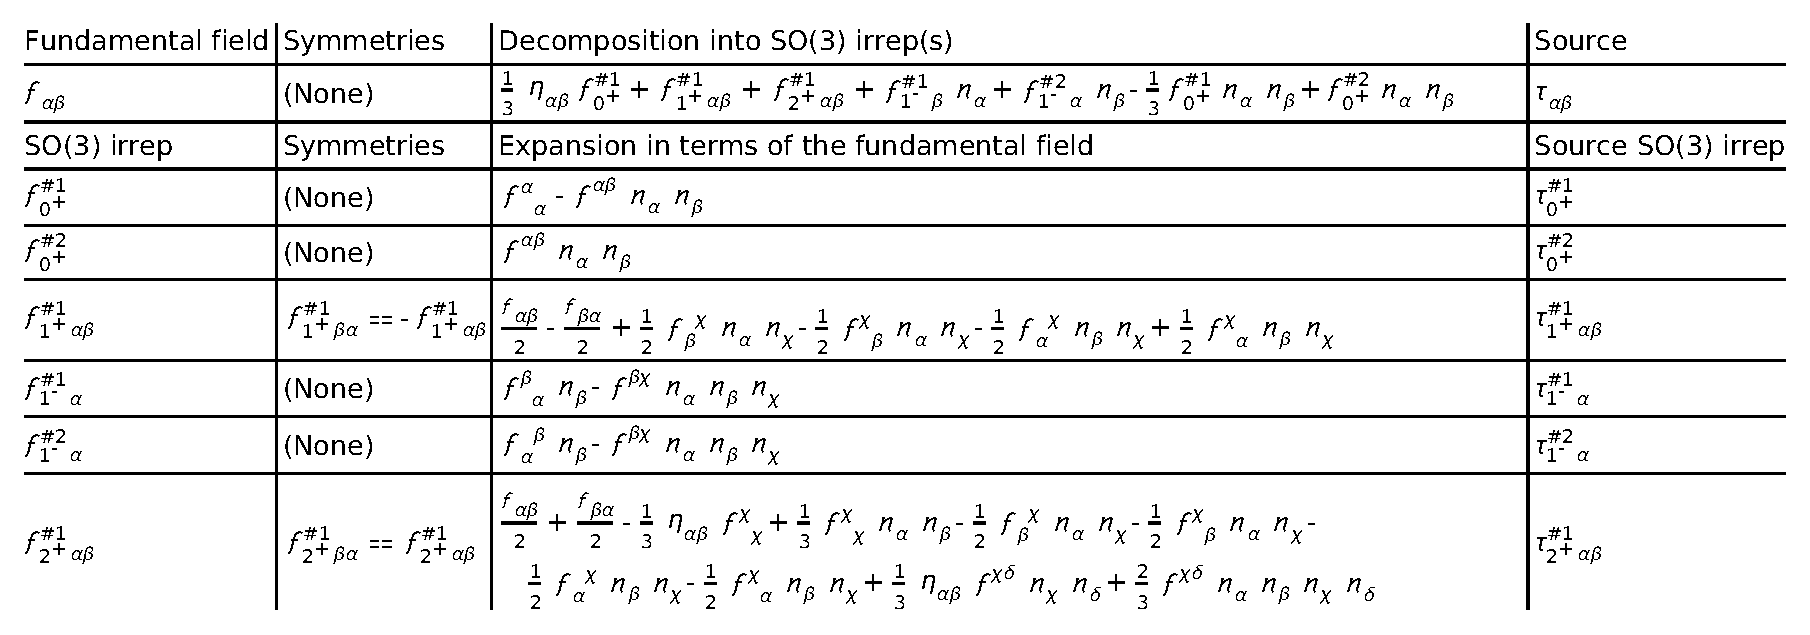
\includegraphics[width=\linewidth]{FieldKinematicsTetradPerturbation.pdf}
  \caption{\protect\CLAUD{Decomposition of the tetrad perturbation~$\tensor{f}{_a^\mu}$ into $J^P$ states, generated with \psalter{}~\citep{Barker:2024juc}, together with its conjugate source current, the asymmetric stress--energy tensor~$\tensor{\tau}{^a_\mu}$. Each state is labelled by its $J^P$ and, where a field contains several states with the same~$J^P$, by a number~$\#i$. At this order, Lorentz and coordinate indices are interchangeable. The SPOs separate the perturbation fields into irreducible $\mathrm{SO}(3)$ components of definite spin $J$ and parity $P$ with respect to the unit direction vector defined by the Fourier momentum, $n^\mu \equiv k^\mu/\sqrt{k_\nu k^\nu}$. These components define the $J^P$ sectors used in~\cref{fig:stigma-particle-spectrum}.}}
  \label{tab:field-kinematics-tetrad}
\end{table*}

\begin{table*}[tp]
  \centering
  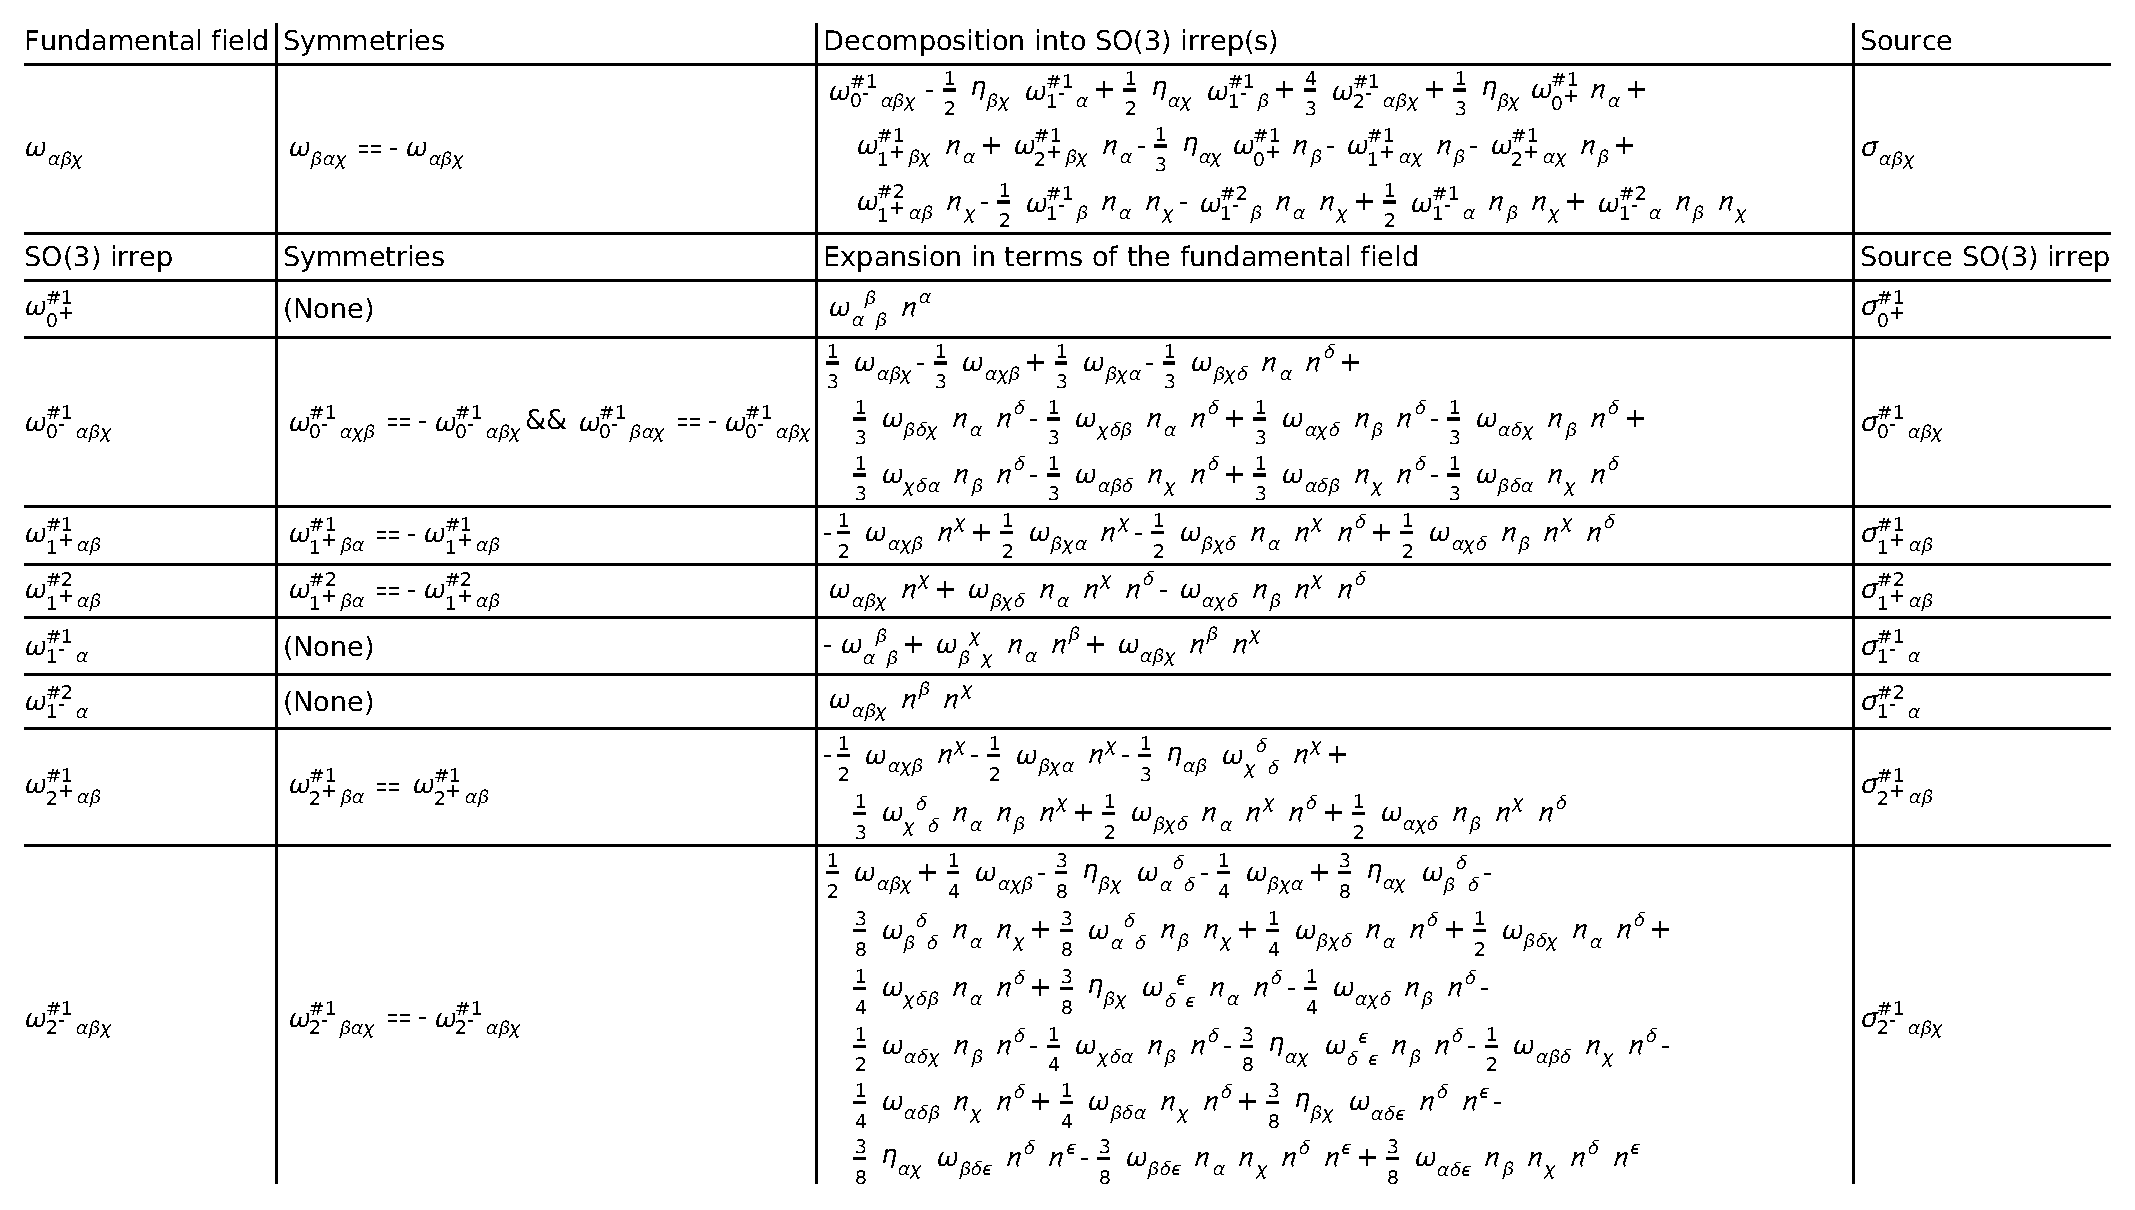
\includegraphics[width=\linewidth]{FieldKinematicsSpinConnection.pdf}
  \caption{\protect\CLAUD{Decomposition of the spin connection~$\tensor{\omega}{^{ab}_\mu}$ into $J^P$ states, generated with \psalter{}~\citep{Barker:2024juc}, together with its conjugate source current, the spin current~$\tensor{\sigma}{_{ab}^\mu}$. These decompositions are performed in the same way as~\cref{tab:field-kinematics-tetrad}.}}
  \label{tab:field-kinematics-spin}
\end{table*}

\subsection{\texorpdfstring{\protect\CLAUD{$\varsigma$TorC}}{sTorC}}
\label{sec:stigma-spectrum}
The linearised form of~\cref{eq:stigma-pgt-lagrangian} depends on the coupling combinations $\sigma_1$, $\sigma_2$, $\upsilon_2$, $\nu$, and $\lambda$. Using $\varsigma=\sigma_1/\sigma_2$, these can equivalently be written in terms of $\varsigma$, $\sigma_2$, $\upsilon_2$, $\nu$, and $\lambda$. Feeding the linearised theory into \psalter{}~\citep{Barker:2024juc,Barker:2025qmw}\CLAUD{, following the same procedure described in~\cref{app:spectrum-method},} produces the particle spectrograph shown in~\cref{fig:stigma-particle-spectrum}. The particle content is the same as for TorC and contains two massless gravitational polarisations and one massive pseudoscalar mode with spin-parity $J^P=0^-$. The massive pseudoscalar has squared mass $m^2=\lambda$, requiring $\lambda\geq0$ to avoid a tachyon, and a residue requiring $\sigma_2<0$ to avoid a ghost. The coupling $\varsigma$ enters the massless sector, requiring $(1+2\varsigma)(\nu+2\varsigma\sigma_2)(\nu-\sigma_2)>0$. Although $\upsilon_2$ appears in the linearised wave operator, it drops out of the physical poles and their residues, and therefore does not give an additional unitarity condition.
Together, these reproduce the unitarity conditions quoted in~\cref{eq:stigma-conditions}.
\begin{figure*}[tp]
  \centering
  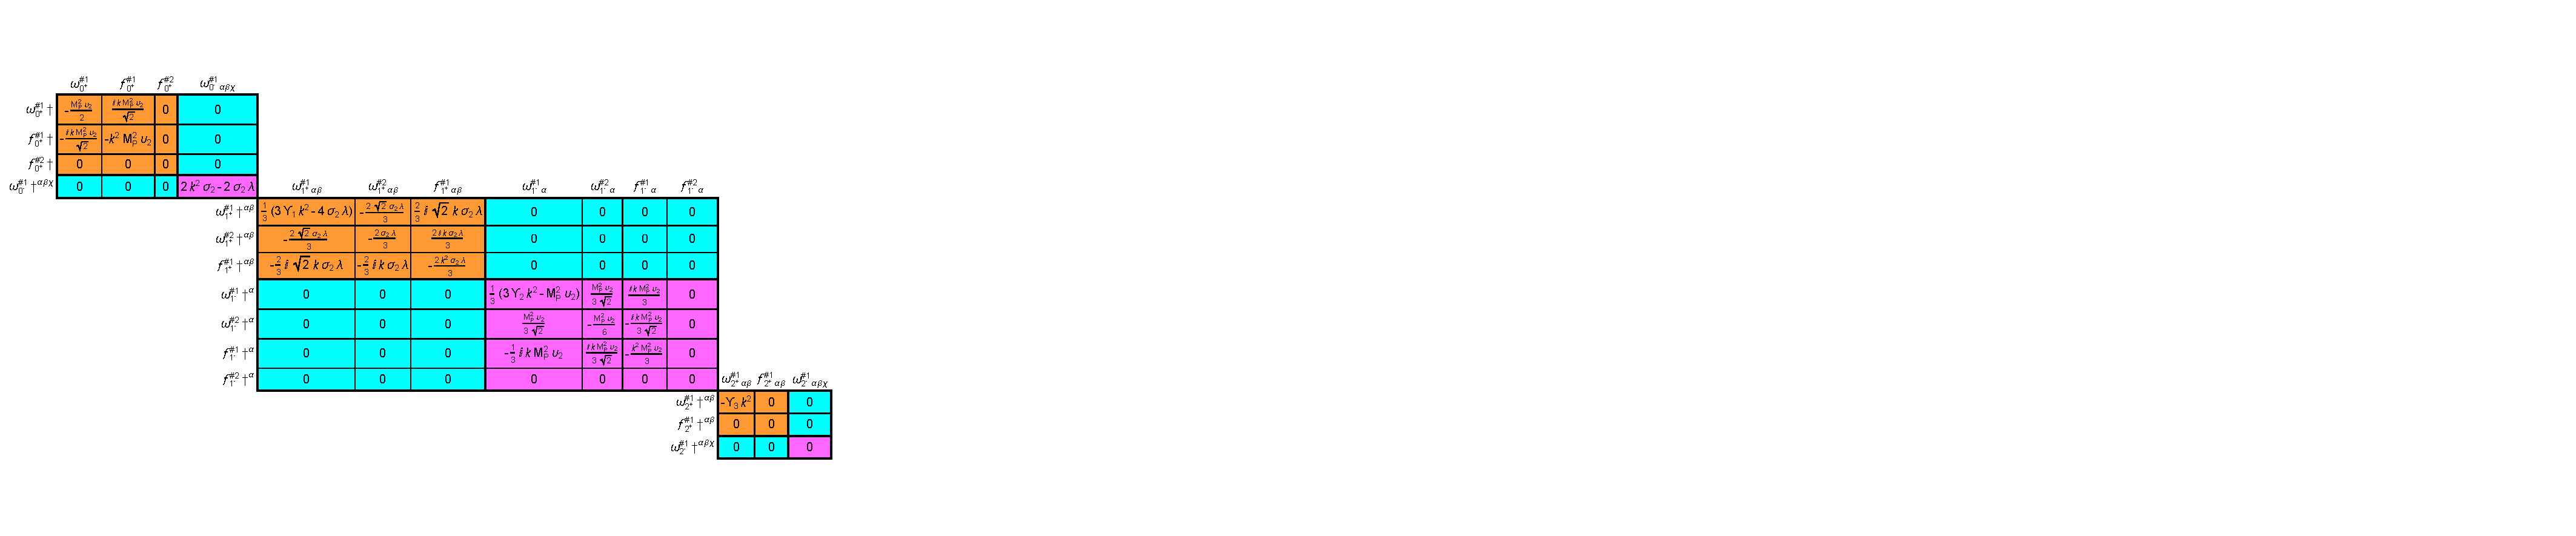
\includegraphics[width=\linewidth]{ParticleSpectrographTorCSigma2NuUpsilon2_1.pdf}\\[0.5\baselineskip]
  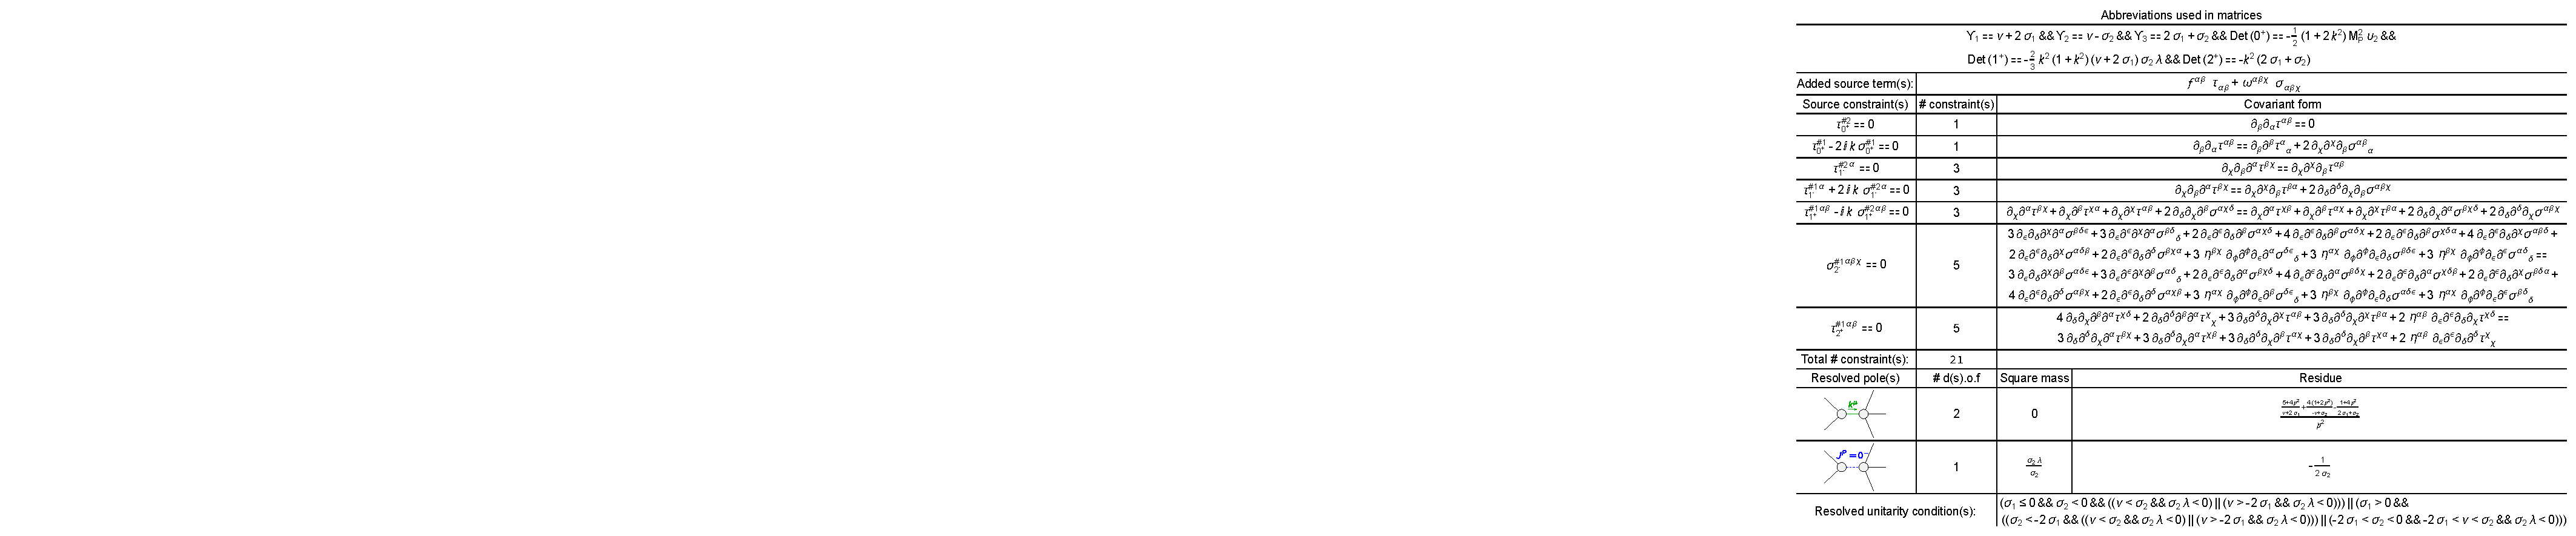
\includegraphics[width=0.9\linewidth]{ParticleSpectrographTorCSigma2NuUpsilon2_2.pdf}
	\caption{Particle spectrum of $\varsigma$TorC generated with \psalter{} for the parameter combination $\sigma_2$, $\varsigma$, $\nu$, $\upsilon_2$, and $\lambda$. \emph{Top:} the blocks of the wave operator\protect\CLAUD{, $\mathsf{O}(k)$ in~\cref{eq:saturated-propagator},} in each spin-parity sector\protect\CLAUD{ defined in~\cref{tab:field-kinematics-tetrad,tab:field-kinematics-spin}}, in the basis of the tetrad and connection perturbations $f$ and $\omega$. The $J^P$ states are separated into blocks of $J=0$, $J=1$, and $J=2$, and further divided into parity-preserving sectors of $P=+1$ (orange) and $P=-1$ (purple), with off-diagonal parity-violating blocks shown in teal. \emph{Bottom:} the abbreviations used in those blocks, the source constraints with their covariant forms, and the resolved poles with their degrees of freedom, square masses and residues, together with the resulting unitarity conditions. There are 21 gauge generators, eleven more than the ten expected from Poincar\'e symmetry. The particle spectrum contains two massless gravitational polarisations and one massive pseudoscalar mode. The massive mode has squared mass $m^2=\lambda$, requiring $\lambda>0$, while its residue requires $\sigma_2<0$. The massless sector requires $(1+2\varsigma)(\nu+2\varsigma\sigma_2)(\nu-\sigma_2)>0$. Together, these reproduce the unitarity conditions quoted in~\cref{eq:stigma-conditions}.}
  \label{fig:stigma-particle-spectrum}
\end{figure*}

\section{$\Omega_\mathrm{m}$--$\varsigma$ posterior distributions}
\label{app:stigma-grids}
\Cref{fig:stigma-grid-om-stigma} shows the $\Omega_\mathrm{m}$--$\varsigma$ posterior distributions for the same dataset and model combinations as~\cref{fig:stigma-grid-om-h0rd}. The three $\varsigma$TorC models show a negative relationship between $\Omega_\mathrm{m}$ and $\varsigma$, consistent with the discussion in~\cref{sec:stigma-effects}. The $\lambda$-only case shows posteriors that are compressed towards lower values of $\Omega_\mathrm{m}$, particularly when DES5Y is included. This reflects the joint dependencies of $\lambda$ on $\varsigma$ through its modification of $\varpi^2$, as discussed in~\cref{sec:stigma-effects}.
\begin{figure*}[tp]
\centering
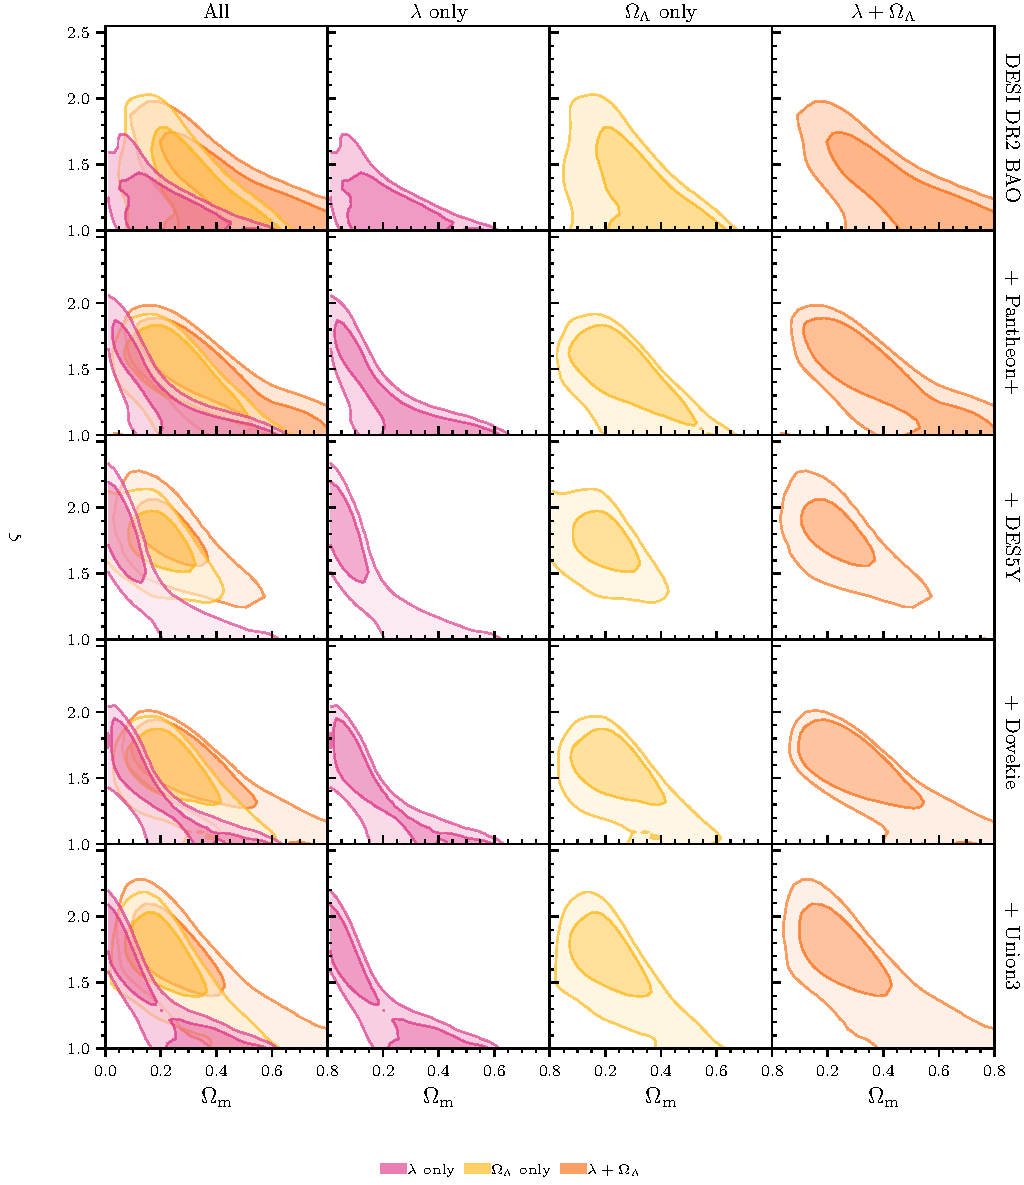
\includegraphics[width=\textwidth]{grid_om_stigma.pdf}
\caption{Posterior distributions in the $\Om$--$\varsigma$ plane, plotted in the same style as~\cref{fig:stigma-grid-om-h0rd}. The figure shows the posterior distribution of the $\lambda$-only (pink), $\Omega_\Lambda$-only (yellow), and the combined $\lambda$ and $\Omega_\Lambda$ (orange) $\varsigma$TorC models. The columns show all three $\varsigma$TorC models, then $\lambda$ only, $\OL$ only, and $\lambda + \OL$, respectively, and the rows show the data sets with DESI DR2 BAO alone, and DESI DR2 BAO combined with Pantheon+, DES5Y, \protect\CLAUD{DES-Dovekie,} and with Union3 individually.}
\label{fig:stigma-grid-om-stigma}
\end{figure*}

\end{document}
